% ELIFE ARTICLE TEMPLATE
% PREAMBLE 
\documentclass[9pt,lineno]{elife}
% Use the onehalfspacing option for 1.5 line spacing
% Use the doublespacing option for 2.0 line spacing
% Please note that these options may affect formatting.
% Additionally, the use of the \newcommand function should be limited.

% ----------------------------------
% \usepackage{lipsum} % Required to insert dummy text
\usepackage[version=4]{mhchem}
\usepackage{siunitx}
\DeclareSIUnit\Molar{M}
% ----------------------------------

% ----------------------------------
\DeclareMathOperator*{\argmax}{argmax} 
\newtheorem{axiom}{Axiom} 
\newtheorem{theorem}{Theorem}
\newtheorem{conjecture}{Conjecture}
\newtheorem{definition}{Definition}
% ----------------------------------

% --------------------------------------------------------------------
% --------------------------------------------------------------------
% --------------------------------------------------------------------
\title{Curiosity is an optimal solution to the exploration-exploitation dilemma}
\author[1,2*]{Erik J Peterson}
\author[1,2,3,4]{Timothy D Verstynen}
\affil[1]{Department of Psychology}
\affil[2]{Center for the Neural Basis of Cognition} 
\affil[3]{Carnegie Mellon Neuroscience Institute}
\affil[4]{Biomedical Engineering, Carnegie Mellon University, Pittsburgh PA}
\corr{Erik.Exists@gmail.com}{EJP}
% \presentadd[\authfn{1}]{Department, Institute, Country}
% \presentadd[\authfn{4}]{Department, Institute, Country}
% \presentadd[\authfn{5}]{eLife Sciences editorial Office, eLife Sciences, Cambridge, United Kingdom}

\begin{document}
\maketitle
\begin{abstract}
We have solved the exploration-exploitation dilemma by joining curiosity learning and reward learning into a single theory. We prove mathematically this theory offers a maximum value solution. This is despite such a solution to the dilemma being impossible for reward learning alone. In simulation--using classic bandit tasks--we surpass standard reinforcement learning in learning tasks where rewards are sparse, or deceptive. 
\end{abstract}

% --------------------------------------------------------------------
% --------------------------------------------------------------------
% --------------------------------------------------------------------
\section{Introduction}
We've been using reinforcement learning to describe animal behavior for almost as long as we've been scientifically studying animal behavior. In its very definition though reinforcement learning leads itself into a dilemma, that cannot be solved. This makes the decision to explore in reinforcement learning into a perennially open theoretical problem.

We think the dilemma is not a fundmental problem. It's that reinforcement learning is a fundamentally incomplete idea. 

What follows is a new formal account of curiosity. It's also a mathematical exploration of three conjectures about how information, exploration, and reward relate. All of these parts let us unify reward learning and curiosity into one theory that can ensure a perfect maximum value solution to the exploration-exploitation dilemma.

% --------------------------------------------------------------------
% --------------------------------------------------------------------
% --------------------------------------------------------------------
\section{Results}
% \begin{figure}
% \begin{fullwidth}
% \includegraphics[width=0.95\linewidth]{elife-18156-fig2}
% \caption{A very wide figure that takes up the entire page, including the gutter space.}
% \label{fig:fullwidth}
% \figsupp{There is no limit on the number of Figure Supplements for any one primary figure. Each figure supplement should be clearly labelled, Figure 1--Figure Supplement 1, Figure 1--Figure Supplement 2, Figure 2--Figure Supplement 1 and so on, and have a short title (and optional legend). Figure Supplements should be referred to in the legend of the associated primary figure, and should also be listed at the end of the article text file.}{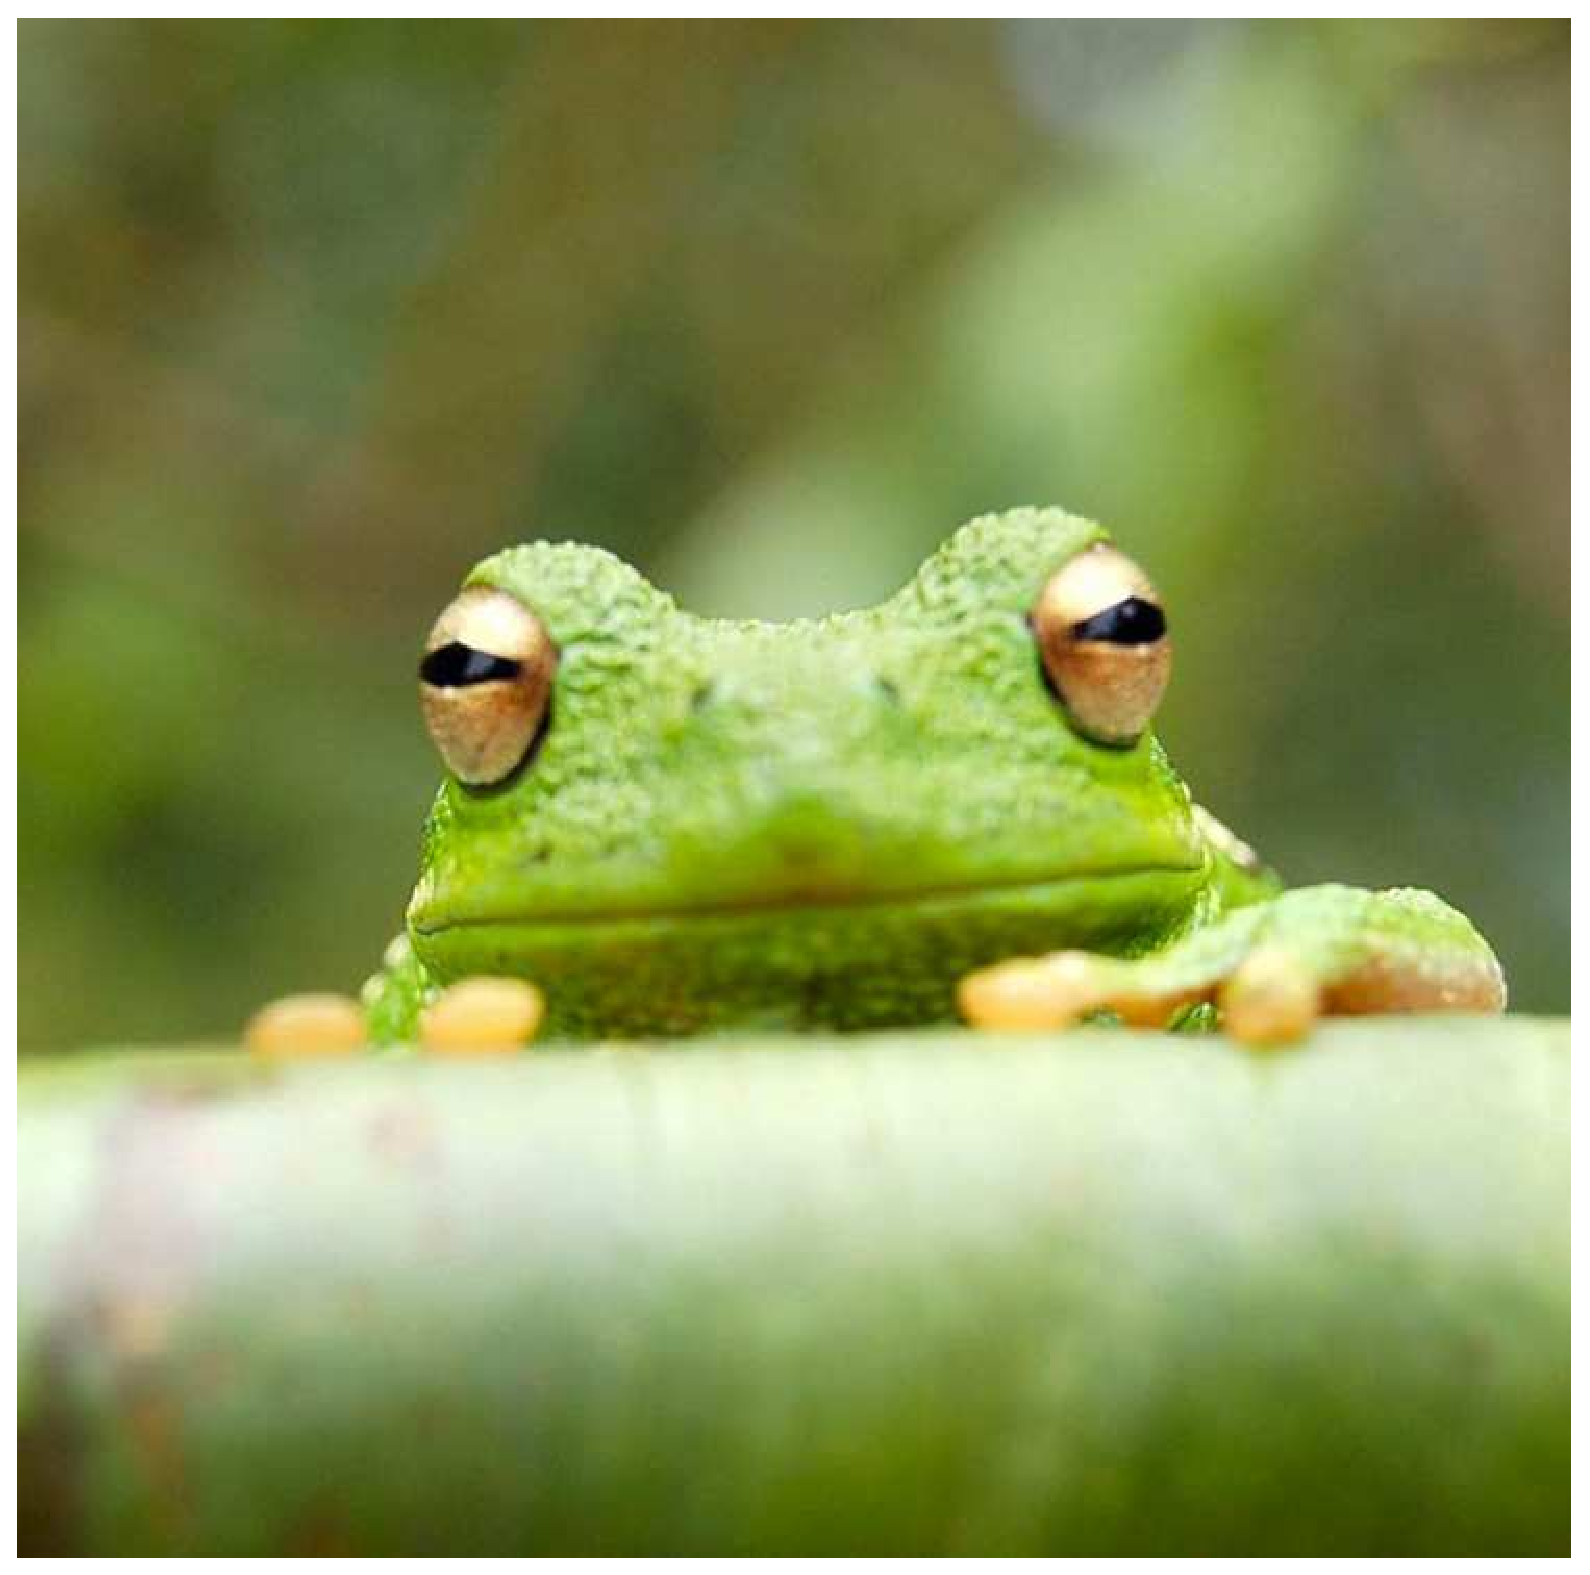
\includegraphics[width=5cm]{frog}}
% \end{fullwidth}
% \end{figure}
% Bacteria have complex receptors designed to sense the gradients of range of chemicals. They have a far broader range than would be needed just to sense food. Curiosity is, we argue, the natural behavioral expression of this. No matter the exact composition of senses, animals have senses which are broadly tuned to understand the environment. The questions as we see it in this paper is how to take the basic fact and necessity of curiosity, as product of general sensors, and make it into something precise and useful mathematically. With that done we can try to make sense theoretically out of the conflicting drives most animals will feel between the drive to learn generally, and collect resources specifically.

% To make it clear exactly how these drives conflict we'll review the exploration-exploitation dilemma as it's generally stated. Then we'll review, and find new holes in, some standard ways to resolve the dilemma. This set the stage for revisiting exploration, as a whole.

\subsection{The dilemma problem}
To explain the dilemma let's look at the problem's extremes. If all an animal wants to do is find the best rewards, from a mathematical point of view the solution is simple. \cite{gittins1974dynamic} proved that the optimal policy for reward collections is one that calculates the expected total future from each possible action, and selects the action with the highest expected reward. Work by \cite{Kearns2002} improved on this basic idea and showed how to find a solution in polynomial time, and \cite{Brafman2002} improved it further still. 

In the same vein as the last paragraph, if all an animal wants to do is to explore the environment, what we will call \textit{open-ended exploration}, then there a range of methods to explore that work quite well in practice \citep{Sutton1990,dayan1996exploration,Sutton1998-kw,daw2006cortical,findling2018computational,Friston2016}. This is despite the fact an optimal solution to exploration is not well established, in a formal sense anyway. 

The difficulty with exploration and exploitation is really in balancing them. In trying to do both, when only one action can be taken at a time. From this point of view, the decision to explore comes with the real risk of getting less. To see how let's imagine a bee who is foraging in a meadow (Figure~\ref{fig:bee}\textbf{A}). Upon entering the meadow, the bee could decide to go to the location of a flower where it has been before. In this scenario the bee is \textit{exploiting} its prior knowledge about a desirable outcome of some nectar. On the other hand, the bee \textit{explore} other locations in the meadow it has not been to before, or has no prior knowledge about. While exploration could lead to finding plants with more nectar, it also comes at a risk finding for example no nectar at all. Optimally managing this risk, which is the same as ensuring maximum value, has been proven to be a mathematically intractable problem \citep{Thrun1992a,Dayan1996,findling2018computational,gershman2018deconstructing}. To see why intuitively consider the problem of a dark hallway. At the end, could be anything. The lack of a rational basis for choosing between the known and the unknown means decision to explore or exploit becomes a dilemma, formally speaking.


\begin{figure}
	[tbhp] \centering 
	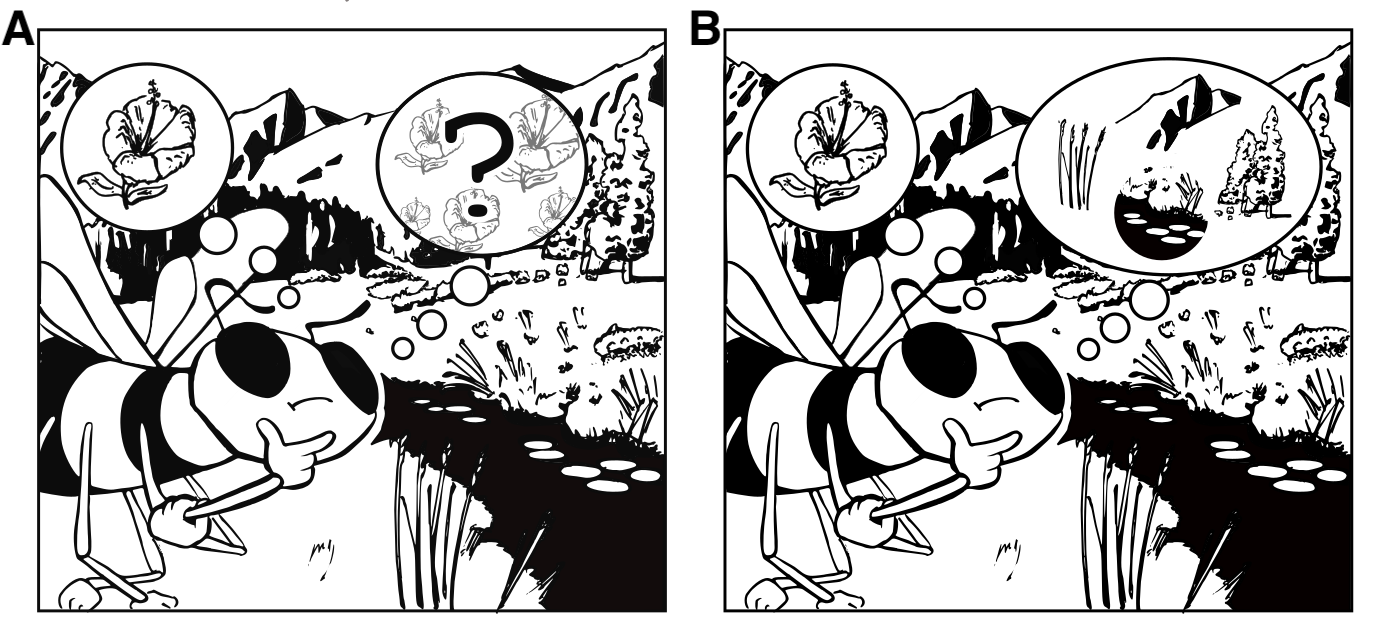
\includegraphics[width=.8\linewidth]{figures/fig1.png} 
	\caption{Two views of exploration and exploitation. \textbf{A}. The classic dilemma: either exploit an action with a known reward (e.g., return to the previous plant) or explore other actions on the chance they will return a better outcome (e.g., find a plant with more flowers). \textbf{B.} Here we offer an alternative view of the dilemma, with two different competitive goals: maximize rewards (e.g., keep returning to known flower locations) \texti{or} build a world model by learning new information (e.g., layout of the environment). Exploration here focused on learning in general, not on reward learning specifically. \textit{Artist credit}: Richard Grant.}
	\label{fig:f1} 
\end{figure}


\subsection*{Intrinsic reward}
Here is a common was to try and solve the dilemma. It is a kind of compromise. It balance rewards with information by treating information as a reward. Intrinsic rewards like these are used both to model animal behavior, and to effectively drive learning in artificial agents. In the next section we'll prove at its heart intrinsic rewards are a contradiction. In this section, we review the basic idea.

The idea behind intrinsic rewards is that if something is valuable, it can be considered a reward, and that we can and should optimize for both tangible rewards, like food and water, along with intrinsic rewards, like information, in the same equation. For example, Eq~\ref{eq:shaping}. 

\begin{equation}
\label{eq:shaping}
\argmax_{\hat \pi} \sum_T R + \beta I
\end{equation}

\begin{equation}
\label{eq:R}
\argmax_{\pi} \sum_T R 
\end{equation}

Recall the goal in the dilemma problem, as we have stated it, is to maximize tangible rewards (Eq~\ref{eq:R}). So if we use information, or intrinsic rewards, to help do that we ideally want them to improve exploration but not hinder exploitation. Let's formalize this idea.

\subsubsection{Formality}
Lets define time $T$ to be on finite horizon, knowing we can extend what followed to an infinite horizon. Let's set reward $R$ to be a real number, and create a function $I$ as a stand in for any intrinsically generated reward. The only thing we'll require of $I$ is that it learns with time. This learning could be about the environment $S$, past or future actions $A$ or past or future rewards. It does not matter for our purposes what the information is about, only that it is learned. We also introduce, as is standard, a free parameter $\beta$ to rescale $I$ as needed. If the final learned action policy $\pi$ is optimal, in some way, for Eq~\ref{eq:R}, we want it be the same policy we would arrive at if we used Eq.~\ref{eq:shaping} in its place. That is, if $\hat \pi$ is the policy we learn using Eq~\ref{eq:shaping} we need $\hat pi = \pi$. This and only this can ensure intrinsic rewards don't alter, or hinder, the final exploitation policy.

\subsection*{Intrinsic bias}
Ideally intrinsic rewards would shape exploration usefully, but that will not bias the final result. The goal is after all to maximize rewards and resources collected in the long term. 

Let's call any bias we find because of a ``bad'' $I$, exploration bias. Formally this means ensuring that a policy that is optimal for $\sum R$ is also optimal for $\sum R + \beta I$. Ng \textit{et al} \cite{Ng1999} studied a related problem to ours, and proved there is only one way to do that.

\cite{Ng1999} proved the only way to safely shape exploration is for $I$ to be what they called a potential function. Well call this $P$ (Eq.~\ref{eq:potential}). In a potential function any cycle of choices, say moving from state $s$ to $s'$ then from $s'$ back to $s$, has a shaping value that sums to zero. Their proof is quite strong. They show a potential function is both necessary and sufficient to leave \textit{any} policy unbiased. That is, if we want $\hat pi = \pi$ then $I$ must be $P$.

\begin{equation}
    \label{eq:potential}
    P = \gamma h' - h
\end{equation}

\cite{Ng1999}'s work leaves at least one open question. How can animal learn $P$? Ng working in the field of computer science, designed the environment they wanted to test. This let them design a ``good'' $P$ ahead of time. They then instilled this into their work and agents. Animals in the natural world are not generally so lucky. They need to learn a good $P$ from the environment.

There are a lot of candidates for learning $P$--reward surprisal, state prediction, novelty are examples--but it does not matter which you'd choose. It turns out we can prove there is a contradiction. A function cannot be a learning function and a potential function at the same time.

\begin{theorem}[Exploration bias]
\label{th:potential}
Let any $S$, $A$, $\gamma$ and potential function $P$ (Eq.~\ref{eq:potential}) be given. We say that $\hat h$ is a real valued learning function such that for $i$th repeated observations of the same state $s_i$ drawn from $S$, then $\hat h$ must change with every observation, $\hat h(s_i) \neq \hat h(s_{i+1}) \neq \hat h(s_{i+2}) \neq \ldots$. Then replacing $h$ in definition of $P$ with \textit{any} learning function $\hat h$ will lead to contradiction in $P$.
\end{theorem}


\subsection*{Intrinsic goals}
Let's take the opposite view of \cite{Ng1999}. They assume we don't want $I$ to bias. Let's assume we do want it too. In this case we still need to control though how much that bias is. With Eq.~\ref{eq:shaping} we cannot do that with any fidelity.

To make this last point clear let's say, for example, Eq.~\ref{eq:shaping} at time $t$ with some action $a$ yields a real number. Say it's, 10.234. We can't know what portion of that number came from the environment $R$ and what came from learned information $B$, or what $beta$'s influence was. It could be the reward was 10 and the information value 0.234. Or it could be the other way around. It is not numerically possible to assign credit for some action $a$ to either $R$ or $I$. All we have is their superposition. This is not enough information when the environment is noisy and $I$ learned. In a noisy environment both values end up changing and we can't learn to control this change.

\subsection*{Value conservation}
In the last two sections we pointed out two mathematical problems with intrinsic rewards. Now let's look at things instead from physical first principles. Let's ask a basic question, is information a reward? 

To see how intangible information and tangible rewards are different, let's consider their value conservation rules.

Tangible rewards are a conserved resource, but learned information is not. If a rat shares potato chip with a cage-mate, she must necessarily split up the chip. This leaves less food for herself. But if student shares the latest result from a scientific paper with a lab-mate, they do not necessarily forget some of the result. Often, their understanding and information will improve by sharing. Of course if the information shared is about a reward, that reward might be lost. Secrets can add extra value. Or we can make up rules which pretend information is conserved. Intellectual property being the example. These are exceptions to the rule though. Information and learning is a general sum game. Collecting tangible rewards is zero sum.


\subsection*{A way around the dilemma}
\label{sec:dilemma}
In the last sections we laid out the dilemma, and described limits in current methods for solving it. This sets the stage for new three hypotheses, or in mathematical speak, conjectures. We'll use these to overcome the problems we outlined, and to solve the dilemma problem. We begin with the basic value of curiosity.

In an informal sense, information is clearly valuable.  From the printing press to the internet to the very existence of languages, humans are a species that insists on inventing new ways to learn information. Yet this is not a uniquely human trait. As we note above, most animals are intrinsically curious about their environments \citep{mehlhorn2015unpacking,hughes1997intrinsic, Gottlieb2018, kidd2015psychology}.

Many animals, like bees, explore out of intrinsic curiosity (Figure~\ref{fig:bee}\textbf{B}) \citep{mehlhorn2015unpacking}. This let's them to learn about their environment, developing an internal model that helps them plan actions and make future decisions \citep{Ahilan2019,Poucet1993}. 

\subsection*{Two big conjectures}
Traditional reward or reinforcement learning sets reward as the primary motivator of behavior. Information primacy theory seem to do the opposite and sets information as the primary motivator. Both views seem too extreme, but both are in a sense right. This lead us to make two new conjectures.

\begin{conjecture}
    \label{conj:1}
    Reward value and information value are equally important for survival.
\end{conjecture}

\begin{conjecture}
    \label{conj:2}
    The only exploratory behavior an animal needs is curiosity.
\end{conjecture}

\subsection*{Dual value learning}
In this paper introduce \textit{dual value learning}. It is a direct answer to the exploration-exploitation dilemma. It is a direct answer to the limit on learning good reward shaping. It is a direct answer to purposeful information bias. It can be summarized by a simple statement.

\begin{conjecture}
    \label{conj:3}
    Exploration and exploitation require independent objectives.
\end{conjecture}

Which has the following mathematical expression, Where $\pi_R$ is a policy for exploitation, and $\pi_E$ is the policy for exploration.

\begin{equation}
\label{eq:dualvalue}    
\begin{split}
\argmax_{\pi_R} \sum_T R \\
\argmax_{\pi_E} \sum_T I    
\end{split}
\end{equation}

It might seem that turning one objective (Eq.~\ref{eq:shaping}) into two (Eq~\ref{eq:dualvalue}) would complicate finding a solution. It does the opposite. In this paper we derive an two valued inequality that naturally solves, or really sidesteps, both the dilemma and exploration bias.

\subsection*{A minimal world model}
We have, in short, conjectured that curiosity is a solution to the exploration-exploitation dilemma. The dilemma is problem found in hugely diverse range of fields, including cognitive science, neuroscience, sociology, economics, game theory, and machine learning. So if we're to solve it in all these settings we need an extraordinarily general definition for information value, which is the name we'll give the term we'll use to drive curious behavior.

Our definition of information value is more general (minimal) then any previous attempt. It is more general than information theory, as we don't require or rely on probability theory. All we assume is that animals have some kind of memory. That they learn from experience. And that they can forget what they learned.

To talk about ``memory'' begs the question, ``memory of what?''. To be concrete we'll thinking of all memories as world models. World models are term common in artificial intelligence. They are memories of experience, \textit{with some amount of simplification} \cite{Schmidhuber1991,Ha2018}. They can range from extremely simple novelty signals, to complete detailed memories of life events \cite{Kakade2002,Bellemare2016,Dayan1993,Schmidhuber1991,Pathak2017,Friston2016,Yang2019,Lopes2012Miller1956,Tulving2002,Park2017,Itti2009,Friston2016,Tenenbaum2006,Kingma2013,Ganguli2008,Ha2018,Schmidhuber2015a,Mante2013}. 

\subsubsection*{Formality}
We want to be able to describe curiosity in animals across the animal kingdom from humans, their children, octopi, bees, to Mongolian gerbils. This means defining memory in way that can accommodate this diversity. We do this by imagining memory a little else but a simple set of numbers.

\textit{Preliminaries.} We assume, without loss of generality, that time is a continuous value and denote increases in time using the differential quantity $dt$. We can then express changes in $M$ (our world model, defined below) as a gradient, $\nabla M$. We also assume that observations about the environment $s$ are real numbers sampled from a finite state space $s \in S$, whose size is $N$ (denoted $S^N$). Actions are also real numbers $a$, drawn from a finite space $A^K$. Rewards $R_t$ -- when they appear -- are binary $(0,1)$ and are provided \textit{only} by the external environment. 

\begin{definition}[Memory]
We define a memory $M$ as a finite set of real numbers, whose maximum size is $L$ ($M^L$). We say that memory has a pair of functions $f$ and $g$. Learning of $s$ at time $t$ (i.e. $s_t$) by $M$ is done by the invertible encoder function $f$, $M_{t+dt} = f(M_{t}, s_{t})$ and $M_{t} = f^{-1}(M_{t+dt}, s_{t})$. Memories $\hat s_t$ about $s_t$ are recalled by the decoder function $g$, $\hat s_t = g(M_t, s_t)$. 
\end{definition}

The invertibility of $f$, denoted as $f^{-1}$, is a mathematical way to ensure that any observations encoded in the world model can also be forgotten. This is both an important aspect of real memory, and a critical point for our mathematical analysis.

The details of $f$ and $g$ define what kind of world model or memory $M$ is. Let's consider some examples. If $f$ adds states $s_t$ to the memory, and $g$ tests whether $s_t$ is in $M$, then $M$ is a model of novelty \cite{Kakade2002}. If $f$ counts states and $g$ returns those counts, then $M$ is a count-based heuristic \cite{Bellemare2016,Dayan1993}. If $f$ follows Bayes rule and $g$ decodes the probability of $s_t$, then $M$ is a Bayesian memory \cite{Itti2009,Friston2016,Tenenbaum2006,Schmidhuber1991,Pathak2017,Friston2016}. If the size of $M$ is much smaller than the size of the state space $S^N$, then $f$ can be seen as learning a latent or compressed representation im $M$ \cite{Kingma2013,Schmidhuber2008,Levi-Aharoni2019,Ganguli2010,Ha2018,Schmidhuber2015a,Mante2013,Park2017}, and $g$ decodes a reconstruction of $s$ ($\hat s_t$) or future states ($\hat s_{t+dt}$).
 
\subsection*{A geometry for information value}
We need to derive a general way to value any piece of information, given a memory $M$. To ensure the definition can span disciplines we take an axiomatic approach, thinking about the problem geometrically.

It might seem strange to think about exploration, memory, and learning as problems in geometry. If we think about life as a path made of steps defined by choices, each choice with its own angle and distance in mental space, the question we can ask is, \textit{when exploring, what is the best next mental step to take?}. We argue that it is the biggest step. An animal should take the action, small or large, that changes its memory the most. Thinking about the problem this way makes the best learners into the best explorers.

\begin{axiom}[Axiom of Change]
\label{ax:1}
    The value of information $E(s_t)$ depends only on the total distance $M$ moves by making observation $s_t$.
\end{axiom}

\noindent Axiom~\ref{ax:1} does three important things. It ensures information value depends only on the world model, that value is a distance in memory, and that value learning has the Markov property \cite{Sutton2018}. 

Unpacking this a little bit more, by distance we mean.

\begin{definition}[Distance]
\label{def:d}
By distance in Ax.~\ref{ax:1} we mean a function $\delta = d(m,m')$, where $m \in M$ and $m' \in M'$ are discrete memories drawn from two memories $M$ and $M'$. We define $d$ so $d \ge 0$ for all $s \in S$, and let $d = 0$ only if $M = M'$. Our definition of $d$ \textit{does not} require the distance in memories from $M$ to $M'$ be the same as from $M'$ to $M$. Nor for the triangle inequality to hold. 
\end{definition} For the technically inclined, Def.~\ref{def:d} makes $d$ a pre-metric and not formally a distance metric. 

\begin{definition}[Total distance]
\label{def:total}
By total distance we mean the norm $||\Delta||$ of all distances $\Delta = \{\delta_1, \delta_2,...,\delta_L\}$ from two memories $M$ and $M'$ both of size $L$.
\end{definition}

Different $f$ and $g$ pairs will naturally need different ways to measure distances $d$ in $M$. For example, in a novelty world model \cite{Kakade2002} either the hamming or Manhattan distance are applicable and would produce binary distance values, as would a count model \cite{Bellemare2016,Dayan1993}. A latent memory \cite{Schmidhuber1991,Pathak2017} might instead use the euclidean norm of its own error gradient \cite{Pascanu2013}. 

\begin{axiom}
	[Axiom of Equilibrium] To be valuable an observation $s_t$ must be learnable by $M$ 
\label{ax:5} 
\end{axiom}

\noindent By learnable we mean two things. First, with every (re)observation of $s$, $M$ should change. Second, the change in $M$ must eventually reach a learned equilibrium. 

\begin{definition}[Information value] Let any $S$, $A$, $M$ and $d$ be given. We define information value $E$ to be the norm $||\Delta||$ of all distances $\Delta = \{\delta_1, \delta_2,...,\delta_L\}$ on $M$ subject to a constraint on the average gradient of $M$, $\mathbb{E}\big [\nabla^2 M \big ] \leq 0$. 
\end{definition}

% Most attempts to value information rest their definition on information theory. Value might rest on the intrinsic complexity of an observation (i.e., its entropy) \cite{Haarnoja2018} or on its similarity to the environment (i.e., mutual information) \cite{Kolchinsky2018}, or on some other salience signal \cite{Tishby2000}. In our analysis, learning alone drives value. This is because learning might happen on a true world model or with a faulty world model, or be about a fictional narrative. The observation might be simple, or complex. From a subjective point of view, which is the right point of view for value, all of these are the same; value depends only on the total knowledge gained.

The beauty of our geometric definition of information value is that it generalizes all previous definitions\footnote{...As far as we can tell.}. Different choice for $f$ and $g$ pairs will naturally need different ways to measure distances in $M$. For example, in a novelty world model \citep{Kakade2002} either the hamming or Manhattan distance are applicable and would produce binary distance values, as would a count model \citep{Bellemare2016,Dayan1993}. A latent memory \citep{Schmidhuber1991,Pathak2017} might instead use the euclidean norm of its own error gradient \citep{Pascanu2013}. While a probabilistic or Bayesian memory would likely use the Kullback–Leibler (KL) divergence \citep{Park2017,Friston2016}.

Most attempts to value information rest on information theory and assume information value and fidelity are naturally connected. In these accounts value might depend on the intrinsic complexity of an observation (i.e., its entropy) \citep{Haarnoja2018} or on its similarity to the environment (i.e., mutual information) \citep{Kolchinsky2018}, or on some other salience signal \citep{Tishby2000}. In our formalism learning alone drives value. We recognize that equally valuable learning can happen on a true world model, or be about a faulty world model, or be about an entirely fictional narrative. A valuable observation might be simple, or it might be complex. From the subjective point of view of the animal learning--which is the right point of view for value--these kinds of differences don't matter. Information value depends only on the total knowledge gained.

\subsection*{A greedy solution to exploration} 
We've formalized curiosity with the new formal axioms for information value. So how do we maximize information value? 

The simplest solution would be a greedy algorithm, one that chooses the largest value at every timestep. A greedy algorithm seems intuitively like the obvious choice for any problem like this, but that not always so \footnote{We'll be working with an example of this for reward in our \textit{Bandits} simulations}. It can actually be difficult to prove a greedy policy won't in the long-term be suboptimal, even though it seems optimal in the short-term \cite{Roughgarden2019,Bellmann1954}.

We'll can prove a greedy policy for information value is optimal in terms of total value. The problem of maximizing information value, as we'll show, reduces to the Bellman equation \cite{Bellmann1954} and so optimal exploration becomes a problem in approximate dynamic programming. Before moving onto the formality though, let's discuss why our result for exploration might be important. Exploration policies generally fall into one two categories, that we will call heuristics and samplers.

Sampling policies use randomness to ensure information about the environment is maximized. This randomness can be directed by previously learned experience, and is often Bayesian\footnote{Also known as active sampling}, or it can be purely random. For example, the classic e-greedy search algorithm. Directed search is more efficient by having less redundancy in its sampling than pure randomness. But because both methods are based on a random processes. They can only make theoretical guarantees about average values or other aggregate statistics. They also cannot make exact moment-by-moment behavioral predictions. 

Count-based, or other similar heuristics \cite{Bellemare2016}, can be deterministic, but they do not generally consider the value of states in the environment. This means that while they can and do describe aspects of exploration they are also missing an essential element -- learning.

Our result on optimal exploration ensures learning value is maximized, ensures a complete search, and a perfectly efficient search, but does so in a strictly deterministic way. This means moment-by-moment prediction of behavior is possible.

\subsubsection*{Formality}
Motivation out of the way, let's consider our solution. Dynamic programming is a popular optimization method because it guarantees value is maximized. In Theorem~\ref{theorem:opt_sub} (see \textit{Mathematical Appendix}) we prove that our definition of memory has one critical property, optimal substructure, useful in finding an optimal dynamic programming solution \cite{Bellmann1954,Roughgarden2019}. Two others are, $E \ge 0$ and the Markov property \cite{Bellmann1954,Roughgarden2019}. Both are already satisfied by \textit{Axiom 1}. 

Let $\pi$ denote an action policy, a function that takes a state $s$ and returns an action $a$. We let $\delta$ denote the transition function, which takes a state-action pair $(s_{t},a_t)$ and returns a new state, $s_{t+dt}$. This function acts as an abstraction for the actual world. For notational consistency with the standard Bellman approach we also redefine $E(s)$ as a \textit{payoff function}, $F(M_{t}, a_t)$ \cite{Bellmann1954}.
 
\begin{equation}
	\begin{split}\label{eq:payout} 
		F(M_{t}, a_t) = E(s)\\
		\text{subject to the constraints} \\
		a_{t} = \pi(s_t) \\
		s_{t+dt} = \delta(s_{t}, a_t),\\
		M_{t+dt} = f(M_{t}, s_{t}) 
	\end{split}
\end{equation}

\noindent The value function for $F$ is,

\begin{equation}\label{eq:V_E} 
	\begin{split}
		V_{\pi_E}(M_0) = \Big [ \max_{a \in A} \sum_{t=0}^{\infty} F(M_t, a_t) \ \Big | \ M, \ d, \ S \ \Big ]. 
	\end{split}
\end{equation}

\noindent And the recursive Bellman solution to learn this value function is,

\begin{equation}\label{eq:bellman_iter} 
	V^*_{\pi_E}(M_{t}) = F(M_{t}, a_{t}) + \max_{a \in A} \Big [ F(M_{t+dt}, a_t) \Big ].
\end{equation}

\subsection{Optimal exploration}
Can we prove maximizing information value leads to optimal exploration? What can optimal exploration mean mathematically? 

There is no single definition of optimal exploration. As mentioned in Section \ref{sec:dilemma}, exploration in the literature is largely viewed as an intractable problem when framed in terms of reward. This ruled out using reward to define optimal exploration. We proposed here a minimal definition. It uses three basic criteria to establish optimal exploration. We'll use $\pi_E^*$ to denote any policy that can satisfy them.

\begin{definition}
\begin{enumerate}[noitemsep,wide=0pt,leftmargin=\dimexpr\labelwidth+2\labelsep\relax]
    \item Optimal exploration should visit all available states of the environment at least once. 
    \item Optimal exploration should cease only once learning about the environment has plateaued. 
    \item Optimal exploration takes as few steps as possible to achieve criterion 1 and 2.
\end{enumerate}
\end{definition}

\noindent
\textit{Note:} Stronger definitions of optimal exploration might ensure states are explored with the least physical effort, or that while maximizing information value the learning agent should also maximize rewards, or other side goals. 

Maximizing information value does lead to optimal exploration. Axioms 1-2 and Eq.~\ref{eq:bellman_iter} guarantee to optimal exploration of any finite space $S$ (Theorems~\ref{theorem:Z} and~\ref{theorem:convergence}).

\begin{theorem}[State search: breadth] \label{theorem:Z} 
    Let any $S$, $A$, $\pi_E$, $\delta$ be given. A greedy policy $\pi_E$ is the unique deterministic policy that ensures all states in $S$ are visited, such that $Z = S$. 
\end{theorem}

\begin{theorem}[State search: depth] \label{theorem:convergence} 
	 Let any $S$, $A$, $\pi_E$, $\delta$ be given. Assuming a deterministic transition function $\delta$, a greedy policy $\pi_E$ will revisit all $s \in S$ until convergence at $E_t \leq \eta$. 
\end{theorem}


\subsection*{Scheduling a way around the dilemma} 
We will now prove that in terms of total value, when information value drives all exploration the dilemma has a optimal solution. In this section by optimal we mean that exploration is regret-free, and will maximize total value. This proof is valid for (nearly) any reinforcement learning policy.

\begin{equation}\label{eq:V_R} 
	V^{\pi_R}_R(s) = \mathbb{E} \Big [ \sum_{k=0}^{\infty} R_{t+k+1} \big | s = s_t \Big ]
\end{equation}

Remember that \textit{our} goal is to find an algorithm that maximizes the total value of both information and reward value. So we imagine policies for curiosity and exploitation are competing to control behavior. We think of these as two jobs that need to be scheduled in an optimal order. Each job produces non-negative values: $E_t$ for information or $R_t$ for reinforcement learning. Our goal is to find an optimal scheduler. Optimal here means maximizing total value over time.

Let's simplify our assumptions. Let's assume each action takes a constant amount of time. Let's assume actions have no energetic cost, or if they do it is constant. Let's assume any policy can only take one action at a time. 

For most scheduling solutions the value of a job is fixed. This is not true for when learning. Information value must change as learning improves. This could lead to very complex estimation problem. To sidestep that let's focus on the most general setting we can. If one has \textbf{no} prior information about the environment, the best predictor of for the next value is the last value \cite{Hocker2019,Roughgarden2019}. Let's assume this precept holds in all our analysis. 

The optimal solution to a scheduling problem with non-negative values, exclusive jobs, and Markovian state is a greedy algorithm \cite{Bellmann1954,Roughgarden2019}. This is give us Eq.~\ref{eq:pipi}. When there is a tie the default policy is reward maximization. Eq.~\ref{eq:pipi} breaks ties between $R_t$ and $E_t$ in favor of $\pi_R$.

To allow Eq.~\ref{eq:pipi} to achieve a stable solution without optimal exploration (defined in the next section), we introduce a free parameter $\eta$. It is a exploration boredom threshold. Larger values of $\eta$ favor exploitation. Most our proofs require however $\eta = 0$, or is other sufficiently small.

\begin{equation}
\label{eq:pipi} 
	\begin{split}
		\pi_{\pi}(s_t) = 
		\begin{cases}
			\pi^*_E(s_t) & : E_t - \eta > R_t \\
			\pi_R(s_t) & : E_t - \eta \le R_t \\
		\end{cases}
		\\
		\text{subject to the constraints}\\
		R_t \in \mathbb{R} \\
		p(R_t=0) > 0 \\
		E_t - \eta \geq 0 \\
		\text{choose}\ E_0 > 0
	\end{split}
\end{equation}

\begin{theorem}[Total value maximization of $\pi_{\pi}$] \label{theorem:meta_total} 
    \label{theorem:meta} 
	 Let any $S$, $A$, $M$, $\pi_R$, and $\delta$ be given. If $\pi_R$ is defined on a Markov Decisions, then $\pi_\pi$ is Bellman optimal and will maximize total value. 
\end{theorem}

\subsubsection*{Other guarantees.} 
Ensuring total value optimized in Eq.~\ref{eq:pipi} doesn't ensure each policy is optimal. Imagine for example that learning in $M$ is very efficient, But for some reason learning of reward is not. This could mean $\pi_E$ converges before $\pi_R$ has finished learning. As $\pi_E$ is \textit{the} mechanism for exploration, this would be catastrophic.

There is always a terrible $\pi_R$ to make this happen. For example, one that forgets all value after every step. But let's assume a good $\pi^*_R$. One that is known to have some desirable guarantee. Does Eq.~\ref{eq:pipi} ensure $\pi^*_R$ will keep this guarantee?

If $\pi^*_R$ guaranteed to succeed in finite samples, then we can set $\eta$ to zero or small enough. If $\pi^*_R$ is guaranteed to succeed under an infinite horizon then $\eta$ must be exactly zero. In both cases $M$ learning must satisfy a stricter variation of Axiom 2 (Eq.~\ref{eq:ax2strict}). This ensures exploration never precisely stops when $\eta$ is exactly zero.

\begin{equation}
\label{eq:ax2strict}
    \mathbb{E}\big [\nabla^2 M \big ] < 0
\end{equation}

Continual albeit slowing exploration, along with Theorem~\ref{theorem:Z} and \ref{theorem:convergence}, requires any guarantees made by $\pi_R$ will hold in $\pi_{\pi}$. At least those guarantees made for sampling or learning convergence.

\begin{theorem}[Independence policy convergence under $\pi_{\pi}$] \label{theorem:meta} 
	 Let any $S$, $A$, $M$, $\pi_R$, $\pi_E$, and $\delta$ be given. Assuming an infinite time horizon, if $\pi_E$ is optimal and $\pi_R$ is optimal, then $\pi_{\pi}$ is also optimal in the same senses as $\pi_E$ and $\pi_R$. 
\end{theorem}


\subsection*{Details} Readers interested in practical performance will find that in, \textit{Bandits}. In the next few sections we offer a detailed analysis of Eq.~\ref{eq:pipi}, covering a partial analysis of sample complexity, model dynamics, and several key limitations and assumptions. 

\subsubsection*{Initial values and ties} \label{sec:init_ties}
The initial value $E_0$ for $\pi^*_E$ can any positive real number, $E_0 > 0$. That will not change $\pi^*_E$'s long term behavior, \textit{but} different choices for $E_0$ will strongly change the algorithm's short-term behavior. This can be quite important in practice. 

By definition a greedy policy like $\pi^*_E$ does not distinguish between tied values; There after all no mathematical way to rank equal values. Theorems~\ref{theorem:convergence} and~\ref{theorem:Z} ensure any tie breaking strategy is valid, so in the long term the choice is arbitrary. However like the choice of $E_0$ tie breaking will strongly affect the short-term behavior. 

% TODO - need cites or to not claim a literature basis
Take from the literature viable tie breaking strategies taken include, ``take the closest option'', ``repeat the last option'', or ``take the option with the highest marginal likelihood''. We suggest the tie breaking scheme is deterministic to maintain the determinism of the whole theory.

% TODO - rewrite. mutual observation should be core part of the theory.
% Say so here
\subsubsection*{Sample complexity}
The worst case algorithmic run time for Eq~\ref{eq:pipi} is linear and additive in its policies. So if in isolation it takes $T_E$ steps to earn $E_{T} = \sum_{T_E} E$, and $T_R$ steps to earn $r_{T} = \sum_{T_R} R$, then the worst case training time for $\pi_{\pi}$ is $T_E + T_R$. It is worth noting that this is only true if neither policy can learn from the other's actions. There is, however, no reason each policy cannot observe the transitions $(s_t, a_t, R, s_{t+dt})$ caused by the other. If this is allowed, worst case training time improves to $\max(T_E, T_R)$.

\subsubsection*{The rates of exploration and exploitation}
In Theorem~\ref{theorem:meta} we proved that $\pi_{\pi}$ inherits the optimality of policies for both exploration $\pi_E$ and exploitation $\pi_R$ over infinite time horizon. This does proof does not say whether $\pi_{\pi}$ will not alter the rate of convergence of each policy. It will, and we can't say exactly how. 

In the common case where rewards are sparse, exploration will be favored. In the ideal case were rewards are frequent and reliable, $E$ can quickly fall to zero, and exploitation is favored. This all depends though on how $M$, and $d$ are defined. For example a very forgetful memory $M$, or very nonlinear distance $d$, will strongly favor exploration even when rewards seem common and stable.

\subsubsection*{Re-exploration}
The parameter $\eta$ is a real valued hyper-parameter (Eq.~\ref{eq:meta_greedy}). It controls how quickly rewarding behavior will dominate. It also controls how easy it is for exploratory behavior resurface. 

If $E_t < \eta$ then $\pi^*_E$ is said to converge. So $\pi^*_R$ dominates. If $\eta$ is small however, then a small changes in observations about the world will allow $pi_E$ to exert control. For example, a small change likelihood of some state $s$ will often lead a small increase in $E_t$. If $\eta$ is small then $E_t < \eta$ is easy to violate, which let's gain $\pi^*_E$ control. If $\eta$ is large, then of course large $E_t$ are needed. 

%  The worst case algorithmic run time for Eq~\ref{eq:pipi} is linear and additive in its policies. So if in isolation it takes $T_E$ steps to earn $E_{T} = \sum_{T_E} E$, and $T_R$ steps to earn $r_{T} = \sum_{T_R} R$, then the worst case training time for $\pi_{\pi}$ is $T_E + T_R$. It is worth noting that this is only true if neither policy can learn from the other's actions. There is, however, no reason that each policy cannot observe the transitions $(s_t, a_t, R, s_{t+dt})$ caused by the other. If this is allowed, worst case training time improves to $\max(T_E, T_R)$.

% TODO need guidepost.
\subsection*{Bandits} 
If curiosity is an useful optimal solution to exploration-exploitation dilemma it should outperform the standard approaches.

One of the clearest examples of the dilemma in action in the natural world is foraging. When foraging, animals must search the environment and choose between new but uncertain patches of rewards like food or water, or exploit familiar ones. In the laboratory foraging experiments can be done directly, but often enough the problem is reduced to simpler maze problems. Like the T-maze, for example. When the environment is simplified as far as possible, multi-armed bandits are the result.

The only goal in a bandit task is identify the most rewarding choice, or ``arm'', from a generally fixed number of options. The only actions available are to choose an arm, and the observe the result \cite{Sutton2018}.
 
Because bandits are the simplest possible expression of the exploration-exploitation dilemma, they are a good baseline. They also serve as a good indicator of performance in complex environments that are, in way or another, bounded by the dilemma problem.
 
In bandits tasks rewards are provided probabilistically by the environment. Maximizing reward is the main goal. Regret $G$ is a measure that evaluates the cost of exploration. It has the form, $G = \hat V - V_a$ where $\hat V$ is the maximum value observed so far and $V_a$ represents the value found by taking any exploratory action \cite{Sutton2018}. By definition, the maximum value arm is is what one would exploit. An optimal strategy for the exploration-exploitation dilemma will maximize total reward \textit{and} have zero total regret.

We examined performance in four bandits tasks. The first was simple (Bandit I, Fig.~\ref{fig:f2}) designed to confirm agents were working as expected and to gauge baseline performance in simple scenario. The remaining three bandits were challenging, featuring either deceptive rewards, very sparse rewards or high-dimensionality (Bandits II-IV, Fig.~\ref{fig:f2}).

\begin{figure}
	[tbhp] \centering 
	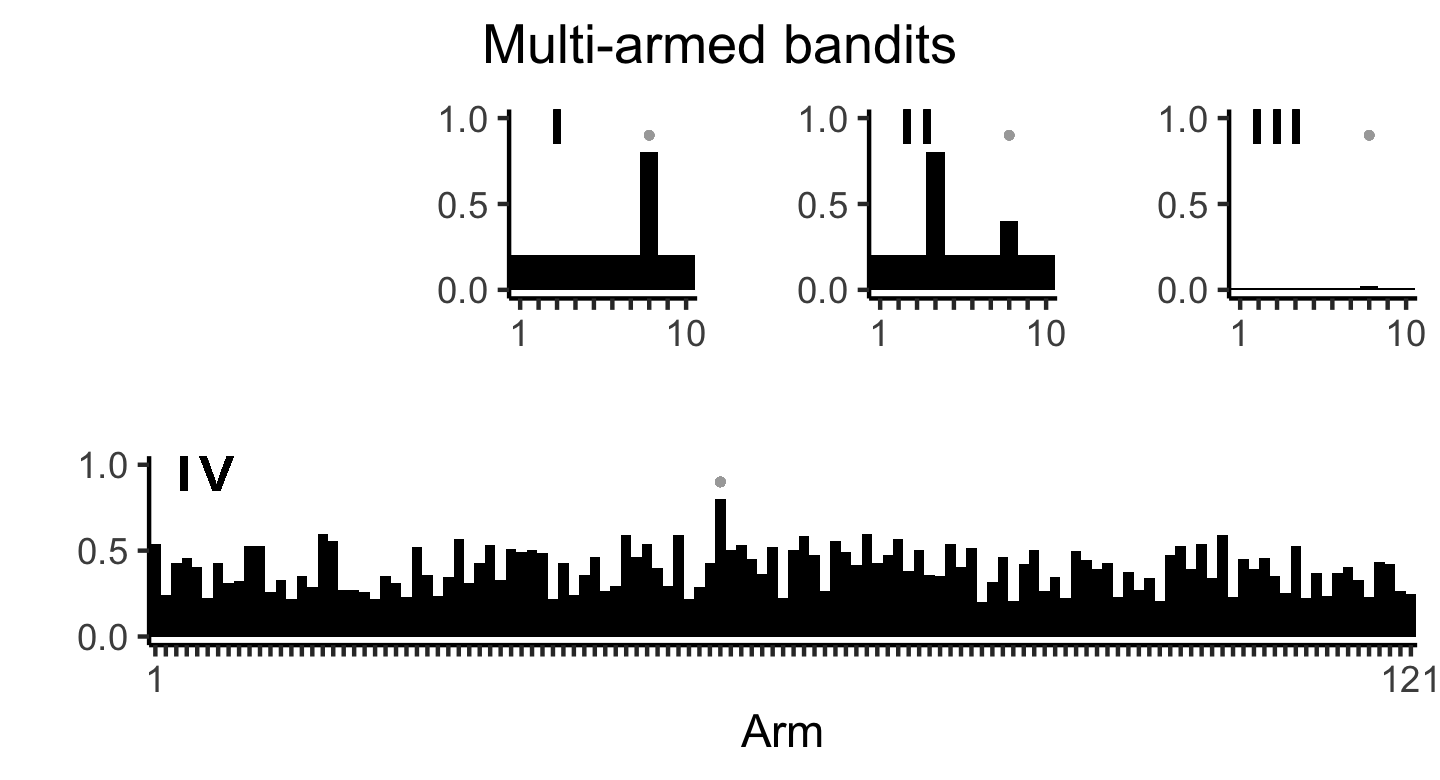
\includegraphics[width=.7\linewidth]{figures/fig2.png} 
	\caption{ \label{fig:f2} Bandits. Reward probabilities for each arm in bandit tasks I-IV. Grey dots highlight the optimal (i.e., highest reward probability) arm. See main text for a complete description.} 
\end{figure}

\begin{figure}
	[tbhp] \centering 
	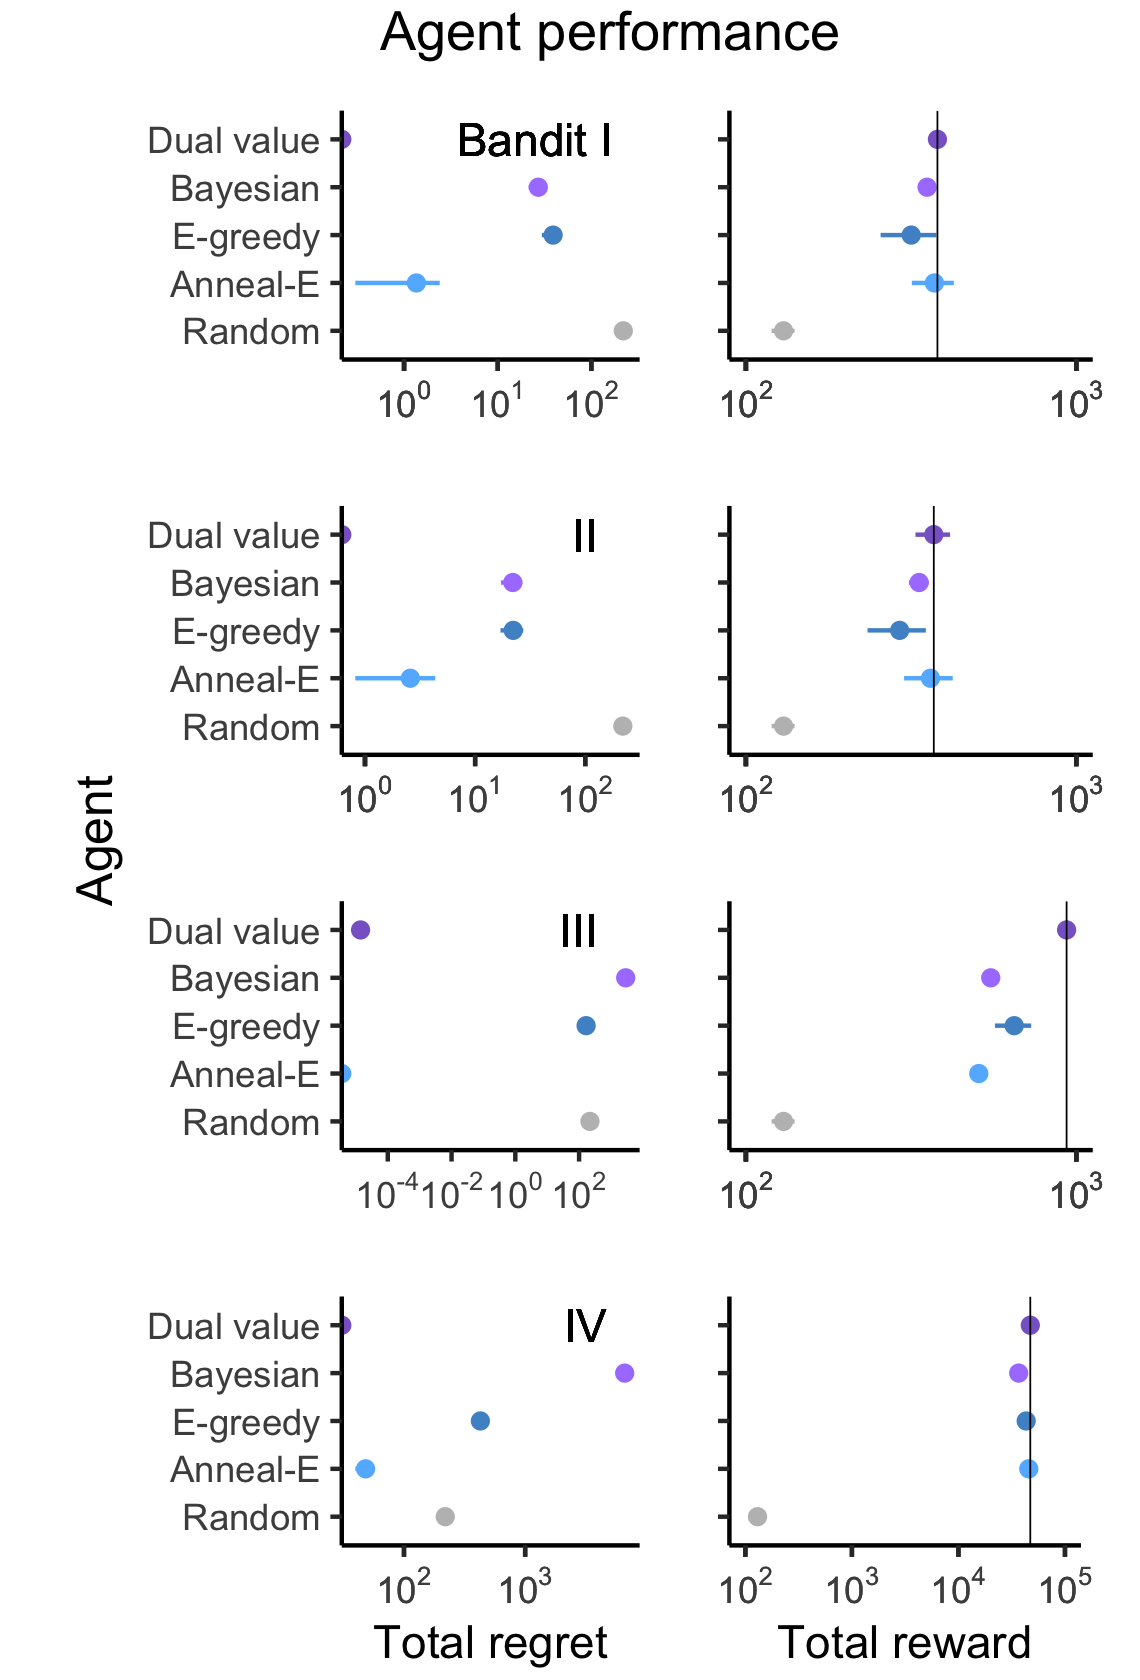
\includegraphics[width=.6\linewidth]{figures/fig3.png} 
	\caption{ \label{fig:f3} Regret and total accumulated reward across models and bandit task. Median total regret (left column) and median total reward (right column) for simulations of each model type ($N=100$ experiments per model). See main text and Table~\ref{tab:agents} for description of each model. Error bars in all plots represent median absolute deviation.} 
\end{figure}

To evaluate dual value learning (Eq.~\ref{eq:pipi}) we compared total reward and regret across a range of both simple, and challenging multi-armed bandit tasks. Despite its apparent simplicity, the essential aspects of the exploration-exploitation dilemma exist in the multi-armed bandit task \cite{Sutton2018}. Here the problem to be learned is the distribution of reward probabilities across arms (Figure ~\ref{fig:f2}).  To estimate the value of any observation $s_t$, we compare sequential changes in this probabilistic memory, $M_{t+dt}$ and $M_t$ using the KL divergence (i.e. relative entropy; Figure \ref{fig:supf1}\textbf{A}-\textbf{B}). The KL divergence is a standard way to measure the distance between two distributions \cite{MacKay2003} and is, by design, consistent with our axioms (see the \textit{Supplementary Materials} for a more thorough discussion). 

We start with a simple experiment involving a single high value arm. The rest of the arms have a uniform reward probability (Bandit \textbf{I}). This represents a trivial problem. Next we tried a basic exploration test (Bandit \textbf{II}), with one winning arm and one distractor arm whose value is close to but less than the optimal choice. We then move on to a more difficult sparse exploration problem (Bandit \textbf{III}), where the world has a single winning arm, but the overall probability of receiving any reward is very low ($p(R) = 0.02$ for the winning arm, $p(R) = 0.01$ for all others). Sparse reward problems are notoriously difficult to solve, and are a common feature of both the real world and artificial environments like Go, chess, and class Atari video games \cite{Mniha,Silver2016b,Silver2018}. Finally, we tested a complex, large world exploration problem (Bandit (\textbf{IV}) with 121 arms, and a complex, randomly generated reward structure. Bandits of this type and size are near the limit of human performance \cite{Wu2018}. 

\subsubsection*{Choice dynamics}. 
The agents in Bandit \textit{I} earned similar amounts of reward (Fig~\ref{fig:f3}, \textit{top row}) but their exploration strategies were quite distinct. In Fig~\ref{fig:supf3}\textbf{B}-\textbf{D}) we compare three prototypical examples -- ours, Bayesian, and E-greedy. This is basic difference hold if all our experiments, and follows from the basic mathematical definitions.

\begin{figure}
	[tbhp] \centering 
	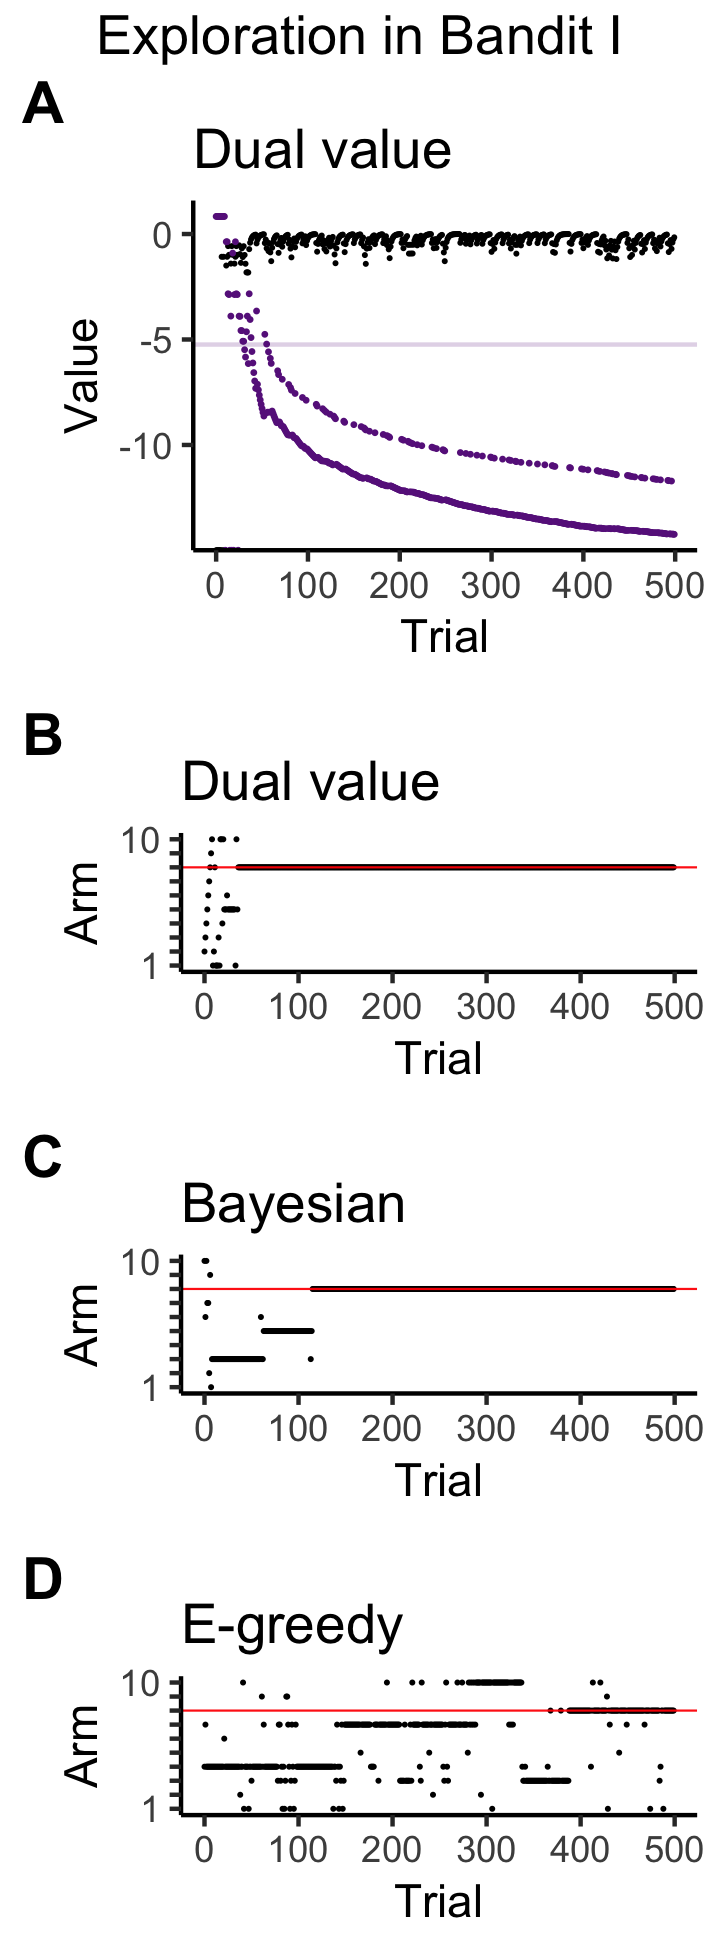
\includegraphics[width=.35\linewidth]{figures/subfig3.png} 
	\caption{\label{fig:supf3} Exploration and value dynamics.
	\textbf{A}. An example of our dual value learning algorithm during 500 trials on Bandit. The light purple line represents the boredom threshold $\eta$ (Eq.~\ref{eq:pipi}).
	\textbf{B.} An example of exploration dynamics (i.e arm selection) on Bandit. Note how the search is structured, and initially sequential.  
	\textbf{C-D.} Exploration dynamics for two other agents. \textbf{C.} The Bayesian agent, which like our algorithm uses active sampling, and values information. Note how this shows a mixture of structures and repeated choices, mixed with seemingly random behavior. \textbf{D.} The E-greedy agent, which uses purely random sampling. Note how here the agent is either greedy, repeating the same arm, or seemingly random.}
\end{figure}

We compared the reward and regret performance of 6 artificial agents. All agents used the same temporal difference learning algorithm (TD(0), \cite{Sutton2018}); see \textit{Supplementary materials}). The only difference between the agents was their exploration mechanism (Table~\ref{tab:agents}). 

The e-greedy algorithm is a classic exploration mechanism \cite{Sutton2018}. Its annealed variant is common in state-of-the-art reinforcement learning papers, like Mnih \emph{et al} (\cite{Mniha}). Other state-of-the-art exploration methods are models that treat Bayesian information gain as an intrinsic reward and the goal of all exploration is to maximize total reward (extrinsic plus intrinsic) \cite{Jaegle2019,Schmidhuber1991}. To provide a lower bound benchmark of performance we included an agent with a purely random exploration policy.

\textit{Note}: Both dual value (ours) and the Bayesian reward algorithm use the KL divergence to estimate information value in a probabilistic space. There are two key differences: 1) Ours has two independent objectives and 2) our makes deterministic choices. Bayesian reward learning by definition relies on random sampling.

\newcolumntype{L}{>{\arraybackslash}m{4cm}} 
\begin{table}[] 
    \centering 
	\caption{Artificial agents.} \label{tab:agents} 
	\begin{tabular}
		{|l|L|} \hline \textbf{Agent} & \textbf{Exploration mechanism} \\
		\hline Dual value & Our algorithm (Eq~\ref{eq:pipi}). \\
		\hline E-greedy & With probability $1-\epsilon$ follow a greedy policy. With probability $\epsilon$ follow a random policy. \\
		\hline Annealed e-greedy & Identical to E-greedy, but $\epsilon$ is decayed at fixed rate. \\
		\hline Bayesian reward & Use the KL divergence as a weighted intrinsic reward, sampling actions by a soft-max policy. $\sum_T R_t + \beta E_t$ \\
		\hline Random & Action are selected with a random policy (no learning) \\
		\hline 
	\end{tabular}
\end{table}

All agents performed well at the different tasks in terms of accumulation of rewards (right column, Figure \ref{fig:f3}). The one exception is the sparse reward task (Bandit III). Here our dual value algorithm consistently returned more rewards than the other models. In contrast, all of the agents but ours had substantial amounts of regret, with partial exception of annealed e-greedy in Bandit III. We say partial because this agent had the worst performance of all learning agents in terms of total rewards. This means its low regret score came from quickly settling on the wrong solution (Figure~\ref{fig:f3})). 

% All of the classic and state-of-the-art algorithms performed well at the different tasks in terms of accumulation of rewards (right column, Figure \ref{fig:f3}). The one exception to this being the sparse low reward probability condition (Bandit \textbf{III}), where the dual value algorithm consistently returned more rewards than the other models. In contrast, most of the traditional models still had substantial amounts of regret in most of the tasks, with the exception of the annealed variant of the e-greedy algorithm during the sparse, low reward probability task (left column, Figure~\ref{fig:f3}). In contrast, the dual value learning algorithm consistently was able to maximize total reward with zero or near zero (Bandit \textbf{III}) regret, as would be expected by an optimal exploration policy.


\subsection*{Reward homeostasis.}
The study of the dilemma often neglects satiety. To simplify the problem its often assumed reward value is constant and that animals are endlessly greedy. This assumption is then often enforced, in a way, by withholding food or water temporarily from animals before an experimental study begins.

Satiety does matter in the natural world, and is key to account for curiosity. Our solution to the dilemma works to this situation, with all its optimality intact. We can show this informally.

In a typical reinforcement learning setting the environment proves the reward and sets it value \cite{Sutton2018}. It's a real number, often just a zero or one. This is the setting Eq.~\ref{eq:pipi} was designed for. It's what we have studied in this paper so far. It's an incomplete picture.

Real animals collecting physical rewards have satiety. They get full, in essence. This is essential for physical animals. They have many competing desires, motivations, and needs. Food, water, sex, and so on. For short, let's call these wants. They also have physical limits to what they can actually consume and do. The value of a reward to animal then depends on the environmental value and their internal state.

Let's call this reward homeostasis, $\hat R$ . Here's a common linear equation for it \cite{burKeramati2014}.

\begin{equation}
\label{eq:homeo}
    \hat R = \bar R - R_t
\end{equation}

Not $R_t$ is the real valued reward from the environment. And we add $\bar R$ which is the reward set point. $\bar R$ is the target for satiety and homeostasis. (We equate the two idea here.) We can put this right into Eq.~\ref{eq:pipi} giving Eq.~\ref{eq:pipi_h1}. 

\begin{equation}
    \label{eq:pipi_h1}
    \begin{split}
		\pi_{\pi}(s_t) = 
		\begin{cases}
			\pi^*_E(s_t) & : E_t - \eta > \bar R - R_t \\
			\pi_{\hat R}(s_t) & : E_t - \eta \le \bar R - R_t \\
		\end{cases}	
	\end{split}
\end{equation}

But if we do put it right in something absurd but important happens when both $E_t - \eta$ and $\bar R - R_t$ are zero or tied. The default when Eq.~\ref{eq:pipi} is tied is to be greedy and gather more rewards. $\pi_R$ wins. This is the exact wrong policy for reward homeostasis. We zero reward in Eq.~\ref{eq:homeo} to prevent exactly this kind of unhelpful gluttony. For Eq.~\ref{eq:pipi_h1} to makes sense we need to break ties in favor of $\pi_E$. This gives us Eq.~\ref{eq:pipi_h2}.

\begin{equation}
    \label{eq:pipi_h2}
    \begin{split}
		\pi_{\pi}(s_t) = 
		\begin{cases}
			\pi^*_E(s_t) & : E_t - \eta \ge \bar R - R_t \\
			\pi_{\hat R}(s_t) & : E_t - \eta < \bar R - R_t \\
		\end{cases}	
	\end{split}
\end{equation}

The one other change we need to make are to the constraints on rewards. In the original we constrain the probability of receiving a reward to greater then one, strictly. This was needed to ensure exploration happens. Now to ensure exploration we need the opposite constraint. We fix $p(R > 0) > 0$. This way reward homeostasis will be reached, eventually. And so exploration will happen, as a result. 

This final equation for $\pi_{\pi}$ under reward homeostasis is.

\begin{equation}
    \label{eq:pipi_h3}
    \begin{split}
		\pi_{\pi}(s_t) = 
		\begin{cases}
			\pi^*_E(s_t) & : E_t - \eta \ge \bar R - R_t \\
			\pi_{\hat R}(s_t) & : E_t - \eta < \bar R - R_t \\
		\end{cases}	
		\\
	    \text{subject to the constraints}\\
		R_t \in \mathbb{R} \\
		p(R_t > 0) > 0 \\
		E_t - \eta \geq 0 \\
		\text{choose}\ E_0 > 0
	\end{split}
\end{equation}

% ---------------------------------------------------------------------
% ---------------------------------------------------------------------
% ---------------------------------------------------------------------
\section*{Discussion}
\subsection*{Past work}
We are not the first to quantify information value \citep{Kolchinsky2018,CogliatiDezza2017}. And we are not the first to use such value to optimize reward collection \citep{Kelly1956,Schmidhuber1991,Dayan1996,deAbril2018,Itti2009}. Information value though is often framed as a means to maximize the amount of tangible rewards (e.g., food, water, money) accrued over time \citep{Sutton2018}. This means that information is treated as an analog of these tangible or external rewards (i.e., an \textit{intrinsic reward}) \citep{Schmidhuber1991,Berger-Tal2014,Itti2009,Friston2016}. This approximation does drive exploration in a practical and useful way. But doesn't change the intractability of the dilemma nor resolve the bias using information can cause \citep{Thrun1992a,Dayan1996,Findling2018,Gershman2018b}. 

% Many accounts of information value rely on both Bayesian reasoning, and information theory \citep{Kelly1956,Itti2009,Friston2016}. In a formal, descriptive, or mathematical world, using these makes sense. However for a naturalistic theory of learning these are strong assumptions, that may not hold up. For example, if it turns out that animals are not in fact general Bayesian reasoning systems. 

At the other extreme from reinforcement learning are pure exploration methods, like curiosity \citep{Berlyne1950,Jaegle2019,Pathak2017} or PAC approaches \citep{Valiant1984}. Curiosity learning is not generally known to converge on rewarding actions with certainty, but never-the-less can be an effective heuristic \citep{Pathak2017,Burda2018,Colas2019}. Within some bounded error, PAC learning is certain to converge \citep{Valiant1984}. For example, it will find the most rewarding arm in a bandit, and do so with a bounded number of samples \citep{Even-Dar2002}. However, the number of samples is fixed and based on the size of the environment (but see \citep{Even-Dar2006,Strehl2009}). So while PAC will give the right answer, eventually, its exploration strategy also guarantees high regret.

\subsection*{Animal behavior}
In psychology and neuroscience, curiosity and reinforcement learning have developed as separate disciplines \citep{Berlyne1950,Kidd2015,Sutton2018}. And they are separate problems, with links to different basic needs: gathering resources to maintain physiological homeostasis \citep{Keramati2014,Juechems2019} and gathering information to plan for the future \citep{Valiant1984,Sutton2018}. Here we suggest that though they are separate problems, they are problems that can, in large part, solve one another.

The theoretical description of exploration in scientific settings is probabilistic \citep{Calhoun2014,Song2019a,Gershman2018b,Schulz2018a}. By definition probabilistic models can't make exact predictions of behavior, only statistical ones. Our approach is deterministic, and so does make exact predictions. Our theory predicts that it should be possible to guide exploration in real-time using, for example, optogenetic methods in neuroscience, or well timed stimulus manipulations in economics or other behavioral sciences. 

\subsection*{Neural systems in simple animals}
% Write about new stuff from Cisek, elegans, and zebrafish
% Cisek (2019) traced the evolution of perception, cognition, and action circuits from the Metazoan to the modern age \citep{Cisek2019}. The circuits for reward exploitation and observation-driven exploration appear to have evolved separately, and act competitively--exactly the model we suggest. In particular he notes that exploration circuits in early animals were closely tied to the primary sense organs (i.e. information) and, historically anyway, had no input from the homeostatic circuits needed for reward valuation \citep{Keramati2014,Cisek2019,Juechems2019}. 


% In species ranging from human to \textit{Caenorhabditis elegans}, there are hundreds perhaps thousands of exploration-exploitation experiments. Analysis of their behavior has been generally been limited to aggregate distributions. A deterministic theory can, in principle, open up entirely new avenues for reanalysis--using our model to make exact temporal predictions.

\subsection*{Artificial intelligence}
Progress in reinforcement learning and artificial intelligence research is limited by three factors: data efficiency, exploration efficiency, and transfer learning \citep{Ha2018}. Our algorithm speaks directly to all three of these limits. By treating exploration as a problem in building a world model, our algorithm always ensures high quality exploration. The focus on the world model also means it can be naturally integrated with data efficient model-based reinforcement learning \citep{Sutton2018,Shyam2018}. Finally, as it builds a world model that is free of any task specific bias and so is ideal for later transfer or fine-tuning \citep{Yosinski2014,Barreto2018}. 

We describe here a simple and optimal algorithm to combine nearly any world model with any reinforcement learning algorithm. This effectively joins the two approaches to reinforcement learning -- model-free and model-based -- into an advantageous whole where exploration is model-based, but exploitation and reward learning is algorithmically model-free.


\subsection*{Energy efficiency}
% TODO - need citations for this whole section.
Energy efficiency is an organizing principle of the nervous system. Determinism and with it greedy information seeking can be seen as extension of that. Each action should try and get the most with each step. This means fewer steps are needed and energy is saved. But what about the energy cost of learning?

Does learning a lot cost the same amount of energy as learning a little? For sparse codes over many cells perhaps so. For small circuits, with only a few cells, sparse has no meaning. So perhaps this changes. For examples see animals like the tunicate and C. elegans.

In some circuits, especially small ones, there might be three part balance. Information gain, balanced by the energetic cost of learning, balanced by the energetic cost of action. Let's leave this to future work. The work we present here is idealized over cost. When learning and action are (nearly) free curiosity and reward collecting are unbounded.

\subsection*{Everyday life} The uncertainty of the unknown can always be recast as an opportunity to learn. But rather than being a trick of positive psychology, we prove this view is (in the narrow sense of our formalism, anyway) mathematically optimal.

% ---------------------------------------------------------------------
% ---------------------------------------------------------------------
% ---------------------------------------------------------------------
\section{Methods and Materials}
\subsection*{Bandits}
Like the slot machines which inspired them, each bandit returns a reward according to a predetermined probability. As an agent can only chose one bandit (``arm'') at a time, so it must decide whether to explore and exploit with each trial.

We study four prototypical bandits. The first has a single winning arm ($p(R) = 0.8$, Figure \ref{fig:f2}\textbf{A}); denoted as bandit \textbf{I}. We expect any learning agent to be able to consistently solve this task. Bandit \textbf{II} has two winning arms. One of these (arm 7, $p(R) = 0.8$) though higher payout than the other (arm 3, $p(R) = 0.6$). The second arm can act as a ``distractor'' leading an to settle on this suboptimal choice. Bandit \textbf{III} also has a single winning arm, but the overall probability of receiving any reward is very low ($p(R) = 0.02$ for the winning arm, $p(R) = 0.01$ for all others). Sparse rewards problems like these are difficult to solve and are common feature of both the real world, and artificial environments like Go, chess, and class Atari video games \citep{Mniha,Silver2016b,Silver2018}. The fourth bandit (\textbf{IV}) has 121 arms, and a complex randomly generated reward structure. Bandits of this type and size are probably at the limit of human performance \citep{Wu2018}. 

\subsection*{$M$ and $d$ for bandits}
All bandits share a simple basic common structure. The have a set of $n$-arms, each of which delivers rewards in a probabilistic fashion. This lends itself to simple discrete n-dimensional world model, with a memory  slot for each arm/dimension. Each slot then represents the independent probability of receiving a reward (Supp. Fig~\ref{fig:supf1}\textbf{A}). 

The Kullback--Leibler divergence (KL) is a widely used information theory metric, which measures the information gained by replacing one distribution with another. It is highly versatile and widely used in machine learning \citep{Goodfellow-et-al-2016}, Bayesian reasoning \citep{Itti2009,Friston2016}, visual neuroscience \citep{Itti2009}, experimental design \citep{Lopez-Fidalgo2007}, compression \citep{Mackay,Still2012} and information geometry \citep{Ay2015}, to name a few examples. KL has seen extensive use in reinforcement learning. % Cites

The Kullback--Leibler ($KL$) divergence satisfies all five value axioms (Eq.~\ref{eq:KL}). 

Itti and Baladi \citepp{Itti2009} developed an approach similar to ours for visual attention, where our information value is identical to their \textit{Bayesian surprise}. Itti and Baladi (2009) showed that compared to range of other theoretical alternative, information value most strongly correlates with eye movements made when humans look at natural images. Again in a Bayesian context, KL plays a key role in guiding \textit{active inference}, a mode of theory where the dogmatic central aim of neural systems is make decisions which minimize free energy \citep{Friston2016,Schwartenbeck2019}. 

\begin{definition}
    Let $E$ represent value of information, such that $E := KL(M_{t+dt}, M_t)$ (Eq.~\ref{eq:KL}) after observing some state $s$.
\end{definition}

\begin{equation}
    KL(M_{t+dt}, M_t) = \sum_{s \in S} M_{t+dt}(s) \text{log} \frac{M_{t+dt}(s)}{M_t(s)} 
    \label{eq:KL}
\end{equation}

Axiom~\ref{ax:1} is naturally satisfied by KL. 

\subsection*{Initializing $\pi_\pi$}
In these simulations we assume that at the start of learning an animal should have a uniform prior over the possible actions $A \in \mathbb{R}^K$. Thus $p(a_k) = 1/K$ for all $a_k \in A$. We transform this uniform prior into the appropriate units for our KL-based $E$ using Shannon entropy, $E_0 = \sum_K p(a_k)\ \text{log}\ p(a_k)$. 

In our simulations we use a tie breaking ``right next'' heuristic which keeps track of past breaks, and in a round robin fashion iterates rightward over the action space.

\subsection*{Reward learning equations} Reinforcement learning in all agent models was done with using the TD(0) learning rule \citep{Sutton2018} (Eq. \ref{eq:TD}). Where $V(s)$ is the value for each state (arm), $\mathbf{R}_t$ is the \emph{return} for the current trial, and $\alpha$ is the learning rate $(0-1]$. See the \emph{Hyperparameter optimization} section for information on how $\alpha$ chosen for each agent and bandit.

\begin{equation}
	\label{eq:TD}
	V(s) = V(s) + \alpha (\mathbf{R}_t - V(s)
\end{equation}

The return $\mathbf{R}_t$ differed between agents. Our dual value agent, and both the variations of the e-greedy algorithm, used the reward from the environment $R_t$ as the return. This value was binary. The Bayesian reward agent used a combination of information value and reward $\mathbf{R}_t = R_t + \beta E_t$, with the weight $\beta$ tuned as described below. 

\subsection*{Hyperparameter optimization}
The hyperparameters for each agent were tuned independently and for each bandit using a random search \citep{Bergstra}. Final values and search ranges are shown in Table~\ref{table:hp}. $N=1000$ samples.

\begin{table}[]
\caption{Hyperparameters for individual bandits (\textbf{I}-\textbf{IV}).}
\label{tab:hp}
\begin{tabular}{|l|l|l|l|l|l|}
\hline
\textbf{Agent} & \textbf{Parameter} & \textbf{I} & \textbf{II} & \textbf{III} & \textbf{IV} \\ \hline
Dual value & $\eta$ & 0.053 & 0.017 & 0.003 & 5.8e-09 \\ \hline
Dual value & $\alpha$ & 0.34 & 0.17 & 0.15 & 0.0011 \\ \hline
E-greedy & $\epsilon$ & 0.14 & 0.039 & 0.12 & 0.41 \\ \hline
E-greedy & $\alpha$ & 0.087 & 0.086 & 0.14 & 0.00048 \\ \hline
Annealed e-greedy & $\tau_E$ & 0.061 & 0.084 & 0.0078 & 0.072 \\ \hline
Annealed e-greedy & $\epsilon$ & 0.45 & 0.98 & 0.85 & 0.51 \\ \hline
Annealed e-greedy & $\alpha$ & 0.14 & 0.19 & 0.173 & 0.00027 \\ \hline
Bayesian & $\beta$ & 0.066 & 0.13 & 0.13 & 2.14 \\ \hline
Bayesian & $\alpha$ & 0.066 & 0.03 & 0.17 & 0.13 \\ \hline
Bayesian & $\gamma$ & 0.13 & 0.98 & 0.081 & 5.045 \\ \hline
\end{tabular}
\end{table}


% -------------------------------------------------------------------
% -------------------------------------------------------------------
% -------------------------------------------------------------------
\section*{Mathematical Appendix.}
\newcommand{\beginsupplement}{%
        \setcounter{table}{0}
        \renewcommand{\thetable}{S\arabic{table}}%
        \setcounter{figure}{0}
        \renewcommand{\thefigure}{S\arabic{figure}}%
     }
\beginsupplement
\setcounter{theorem}{0}

\subsection*{Exploration bias}
\begin{theorem}[Exploration bias]
\label{th:potential}
Let any $S$, $A$, $\gamma$ and potential function $P$ (Eq.~\ref{eq:potential}) be given. We say that $\hat h$ is a real valued learning function such that for $i$th repeated observations of the same state $s_i$ drawn from $S$, then $\hat h$ must change with every observation, $\hat h(s_i) \neq \hat h(s_{i+1}) \neq \hat h(s_{i+2}) \neq \ldots$. Then replacing $h$ in definition of $P$ with \textit{any} learning function $\hat h$ will lead to contradiction in $P$.
\end{theorem}
\begin{proof}
Let $f$ be shaping function where $h$ is any real valued function ($h \in \mathbb{R})$) and $s_1$ and $s_2$ are drawn from a finite state space $S$.

\begin{equation}
\label{supeq:f}
f(s_1,a,s_2) = h(s_2) - h(s_1)    
\end{equation}

Let any function be called a potential function $P(s_1,a,s_2)$ if it returns a real number, and the sum of any cycle of state choices on $S$ is 0 such that if we move from state $s_1$ to $s_2$ giving $P_1$ then back again from $s_2$ to $s_1$ giving $P_2$ then,

\begin{equation}
\label{supeq:P}
P_1 + P_2 = 0.
\end{equation}

Substituting $f$ into both sides for $P_1$ and $P_2$, and rearranging terms, we can show $f$ is a potential function.

\begin{align*}
    P_1               &= -P_2\\
    (h(s_2) - h(s_1)) &= -(h(s_1) - h(s_2))\\
                      &= (h(s_2) - h(s_1))
\end{align*}

Now let $\hat h$ be a learning value function which for repeated observations of the same state $s$, drawn $i$th times from $S$, must change such that $\hat h(s_i, \theta) \neq \hat h(s_{i+1}, \theta) \neq \hat h(s_{i+2}, \theta) \neq \ldots$. 

Without loss of generality we can restrict $\hat h$ to be decreasing such that $\hat h_i > \hat h_{i+1} > \hat h_h_{i+2} > \ldots$ which can be restated for any two sequential pairs as $\hat h_i = \hat h_{i+1} - \delta$, where $\delta$ is a positive real number.

If we then substitute in $\hat h$ for $h$ in Eq.~\ref{supeq:f}, and again rearrange terms through Eq.~\ref{supeq:P}, we find a contradiction, thereby proving a function cannot be learning function and potential function. 

\begin{align*}
    P_1                         &= -P_2\\
    (\hat h(s_2) - \hat h(s_1)) &= -(\hat h(s_1) - \delta - \hat h(s_2))\\
                                &= (\hat h(s_1) - \hat h(s_2) + \delta)
\end{align*}
\end{proof}

\subsection*{Information value as a dynamic programming problem} To find greedy dynamic programming \citep{Roughgarden2019,Sutton2018} answers we must prove our memory $M$ has optimal substructure. By optimal substructure we mean that $M$ can be partitioned into a small number, collection, or series of memories, each of which is itself a dynamic programming solution. In general by proving we can decompose some optimization problem into a small number of sub-problems whose optimal solution are known, or easy to prove, it becomes trivial to prove that we can also grow the series optimally. That is, proving optimal sub-structure nearly automatically allows for proof by induction \citep{Roughgarden2019}. 

\begin{theorem}[Optimal substructure] \label{theorem:opt_sub} 
    Let any $S$, $A$, $M$ (Def. 1), $\pi_E$ and $\delta$ be given. Assuming transition function $\delta$ is deterministic, if $V^*_{\pi_E}$ is the optimal information value given by policy $\pi_E$, a memory $M_{t+dt}$ has optimal substructure if the the last observation $s_t$ can be removed from $M_t$, by $M_{t+dt} = f^{-1}(M_{t+dt}, s_t)$ such that the resulting value $V^*_{t-dt} = V^*_{t} - F(M_t, a_t)$ is also optimal. 
\end{theorem}
\begin{proof}
	Given a known optimal value $V^*$ given by $\pi_E$ we assume for the sake of contradiction there also exists an alternative policy $\hat \pi_E \neq \pi_E$ that gives a memory $\hat M_{t-dt} \neq M_{t-dt}$ and for which $\hat V^*_{t-dt} > V^*_{t-dt}$. 
	
	To recover the known optimal memory $M_t$ we lift $\hat M_{t-dt}$ to $M_t = f(\hat M_{t-dt}, s_t)$. This implies $\hat V^* > V^*$ which in turn contradicts the purported original optimality of $V^*$ and therefore $\hat \pi_E$.
\end{proof}

\subsection*{Bellman solution} Armed with optimal substructure of $M$ we want to do the next natural thing and find a recursive Bellman solution to maximize our value function for $F$ (Eq.~\ref{eq:payout}). (A Bellman solution of $F$ is also a solution for $E$ (Eq.\ref{eq:V_E}). We do this in the classic way by breaking up the series for $F$ into an initial value $F_0$, and the remaining series in the summation. We can then apply this same decomposition recursively (Eq~\ref{eq:bellman_iter}) to arrive at a final ``twp-step'' or recursive form which is shown Eq.~\ref{eq:bellman_seq}). 

\begin{equation}\label{eq:bellman_seq} 
	\begin{split}
		V^*_{\pi_E}(M_0) &= \max_{a \in A} \Big [\sum_{t=0}^{\infty} F(M_t, a_t)\Big ]\\
		&= \max_{a \in A} \Big [F(M_0, a_0) + \sum^{\infty}_{t=1} F(M_{t+dt}, a_{t+dt})\Big ]\\
		&= F(M_0, a_0) + \max_{a \in A} \Big [\sum_{t=1}^{\infty} F(M_{t+dt}, a_{t+dt}) \Big ]\\
		&= F(M_0, a_0) + V^*_{\pi_E}(M_{t+dt}) + V^*_{\pi_E}(M_{t+2}),\ \ldots 
	\end{split}
\end{equation}

\subsection*{A greedy policy explores exhaustively} To prevent any sort of information bias, we need the exploration policy $\pi_E$ (Eq.\ref{eq:bellman_iter}) to visit each state $s$ in the space $S$. We need it to be sure to revisit until learning is dine. As our policy for $E$ is a greedy policy, proving this for exploration amounts to solving sorting problems. 

If a state is to be visited it must have highest value. So if every state must be visited (which is what we need to prove to avoid bias) then under a greedy policy every state's value must, at one time or another, be the maximum value. 

We assume implicitly here the action policy $\pi_E$ can visit all possible states in $S$. If for some reason $\pi_E$ can only visit a subset of $S$ then then the proofs below apply to that subset.

\textbf{Definitions.} Let $Z$ be the set of all visited states, where $Z_0$ is the empty set $\{\}$ and $Z$ is built iteratively over a path $P$, such that $Z_{t+\dt} = \{s | s \in P\ \text{and}\ s \not\in Z_t\}$. 

Sorting requires ranking. So we also need to formalize ranking. We take an algebraic approach and define the following for any three real numbers $(a,b,c)$ (Eq.~\ref{eq:ineq}). 

\begin{align}\label{eq:ineq} 
	a \leq b \Leftrightarrow \exists \ c;\ b = a + c \\
	a > b \Leftrightarrow (a \neq b) \wedge (b \leq a) 
\end{align}

\begin{theorem}[State search: breadth] \label{theorem:Z} 
    Let any $S$, $A$, $\pi_E$, $\delta$ be given. A greedy policy $\pi_E$ is the unique deterministic policy that ensures all states in $S$ are visited, such that $Z = S$. 
\end{theorem}
\begin{proof}
	Let $\mathbf{E} = (E_1, E_2, ...)$ be ranked series of $E$ values for all states $S$, such that $(E_1 \geq E_2, \geq ...)$. To swap any pair of values ($E_i \geq E_j$) so ($E_i \leq E_j$) by Eq.~\ref{eq:ineq} $E_i - c = E_j$. 
	
	Therefore, again by Eq.~\ref{eq:ineq}, $\exists \int \delta E(s) \rightarrow -c$. 
	
	\textit{Recall}: Axiom 2.
	
	However if we wished to instead swap ($E_i \leq E_j$) so ($E_i \geq E_j$) by definition $\not \exists c; E_i + c = E_j$, as $\not \exists \int \delta \rightarrow c$. 
	
	To complete the proof, assume that some policy $\hat \pi_E \neq \pi^*_E$. By definition policy $\hat \pi_E$ can be any action but the maximum, leaving $k-1$ options. Eventually as $t \rightarrow T$ the only possible swap is between the max option and the $kth$, but as we have already proven this is impossible as long as Axiom 2 holds. Therefore, the policy $\hat \pi_E$ will leave at least 1 option unexplored and $S \neq Z$. 
\end{proof}
\begin{theorem}[State search: depth] \label{theorem:convergence} 
	 Let any $S$, $A$, $\pi_E$, $\delta$ be given. Assuming a deterministic transition function $\delta$, a greedy policy $\pi_E$ will revisit all $s \in S$ until convergence at $E_t \leq \eta$. 
\end{theorem}
\begin{proof}
	\textit{Recall}: Axiom 2. Each time $\pi^*_E$ visits a state $s$, so $M \rightarrow M'$, $F(M', a_{t+dt}) < F(M, a_t)$
	
	In Theorem~\ref{theorem:Z} we proved only a deterministic greedy policy will visit each state in $S$ over $T$ trials.
	
	By induction, if $\pi^*E$ will visit all $s \in S$ in $T$ trials, it will revisit them in at most $2T$, therefore as $T \rightarrow \infty$, $E \rightarrow \eta$. 
\end{proof}

\subsection*{Optimality of $\pi_{\pi}$} \label{sec:opt_pipi} 
In the following section we prove two things about the optimality of $\pi_\pi$. First, if $\pi_R$ and/or $\pi_E$ had any optimal asymptotic property for value learning before their inclusion into our scheduler, they retain that optimal property under $\pi_\pi$. Second, we use this Theorem to show if both $\pi_R$ and $\pi_E$ are greedy, and $\pi_\pi$ is greedy, then Eq~\ref{eq:pipi} is certain to maximize total value. This is analogous to the classic activity selection problem \citep{Roughgarden2019}.

\begin{theorem}[Independence policy convergence under $\pi_{\pi}$] \label{theorem:meta} 
	 Let any $S$, $A$, $M$, $\pi_R$, $\pi_E$, and $\delta$ be given. Assuming an infinite time horizon, if $\pi_E$ is optimal and $\pi_R$ is optimal, then $\pi_{\pi}$ is also optimal in the same senses as $\pi_E$ and $\pi_R$. 
\end{theorem}
\begin{proof}
	The optimality of $\pi_{\pi}$ can be seen by direct inspection. If $p(R = 0) > 0$ we are given an infinite horizon, then $\pi_E$ will have a unbounded number of trials meaning the optimally of $P^*$ holds. Likewise, $\sum E < \eta$ as $T \rightarrow \infty$, ensuring $pi_R$ will dominate $\pi_{\pi}$ therefore $\pi_R$ will asymptotically converge to optimal behavior. 
\end{proof}

In proving this optimality of $\pi_{\pi}$ we limit the probability of a positive reward to less than one, denoted by $p(R_t = 1) < 1$. Without this constraint the reward policy $\pi_R$ would always dominate $\pi_{\pi}$ when rewards are certain. While this might be useful in some circumstances, from the point of view $\pi_E$ it is extremely suboptimal. The model would never explore. Limiting $p(R_t = 1) < 1$ is reasonable constraint, as rewards in the real world are rarely certain. A more naturalistic to handle this edge case is to introduce reward satiety, or a model physiological homeostasis \citep{Keramati2014,Juechems2019}.

\subsubsection*{Optimal scheduling for dual value learning problems}
In classic scheduling problems the value of any job is known ahead of time \citep{Bellmann1954,Roughgarden2019}. In our setting, this is not true. Reward value is generated by the environment, \textit{after} taking an action. In a similar vein, information value can only be calculated \textit{after} observing a new state. Yet Eq.~\ref{eq:pipi} must make decisions \textit{before} taking an action. If we had a perfect model of the environment, then we could predict these future values accurately with model-based control. In the general case though we don't what environment to expect, let alone having a perfect model of it. As result, we make a worst-case assumption: the environment can arbitrarily change--bifurcate--at any time. This is, it is a highly nonlinear dynamical system \citep{Strogatz1994}. In such systems, myopic control--using only the most recent value to predict the next value-- is known to be an robust and efficient form of control \citep{Hocker2019}. We therefore assume that last value is the best predictor of the next value, and use this assumption along with Theorem~\ref{theorem:meta} to complete a trivial proof that Eq.~\ref{eq:pipi} maximizes total value.

\subsubsection*{Optimal total value}
If we prove $\pi_{\pi}$ has optimal substructure, then using the same replacement argument \citep{Roughgarden2019} as in Theorem~\ref{theorem:meta}, a greedy policy for $\pi_\pi$ will maximize total value.

\begin{theorem}[Total value maximization of $\pi_{\pi}$] \label{theorem:meta_total} 
    \label{theorem:meta} 
	 Let any $S$, $A$, $M$, $\pi_R$, and $\delta$ be given. If $\pi_R$ is defined on a Markov Decisions, then $\pi_\pi$ is Bellman optimal and will maximize total value. 
\end{theorem}
\begin{proof}
    We assume Reinforcement learning algorithms are embedded in Markov Decisions space, which by definition have optimal substructure.
    
    \textit{Recall}: The memory $M$ has optimal substructure (Theorem~\ref{theorem:opt_sub}.
    
    \textit{Recall}: The asymptotic behavior of $\pi_R$ and $\pi_E$ are independent under $\pi_\pi$ (Theorem~\ref{theorem:meta}
	
	If both $\pi_R$ and $\pi_E$ have optimal substructure, and are asymptotically independent, then $\pi_\pi$ must also have optimal substructure. If $\pi_\pi$ has optimal substructure then it is Bellman optimal.
\end{proof}

% -------------------------------------------------------------------
% -------------------------------------------------------------------
% -------------------------------------------------------------------
\section{Acknowledgments}
EP and TV wish to thank Jack Burgess, Matt Clapp, Kyle ``Donovank'' Dunovan, Richard Gao, Roberta Klatzky, Jayanth Koushik, Alp Muyesser, Jonathan Rubin, and Rachel Storer for their comments on earlier drafts. EP also wishes to thank Richard Grant for his illustration work in Figure 1.

The research was sponsored by the Air Force Research Laboratory (AFRL/AFOSR) award FA9550-18-1-0251. The views and conclusions contained in this document are those of the authors and should not be interpreted as representing the official policies, either expressed or implied, of the Army Research Laboratory or the U.S. government. TV was supported by the Pennsylvania Department of Health Formula Award SAP4100062201, and National Science Foundation CAREER Award 1351748.


% \nocite{*} % This command displays all refs in the bib file. PLEASE DELETE IT BEFORE YOU SUBMIT YOUR MANUSCRIPT!
\bibliography{library}

%%%%%%%%%%%%%%%%%%%%%%%%%%%%%%%%%%%%%%%%%%%%%%%%%%%%%%%%%%%%
%%% APPENDICES
%%%%%%%%%%%%%%%%%%%%%%%%%%%%%%%%%%%%%%%%%%%%%%%%%%%%%%%%%%%%

% \appendix
% \begin{appendixbox}
% \label{first:app}
% \section{Firstly}
% \lipsum[1]

% %% Sadly, we can't use floats in the appendix boxes. So they don't "float", but use \captionof{figure}{...} and \captionof{table}{...} to get them properly caption.
% \begin{center}
% 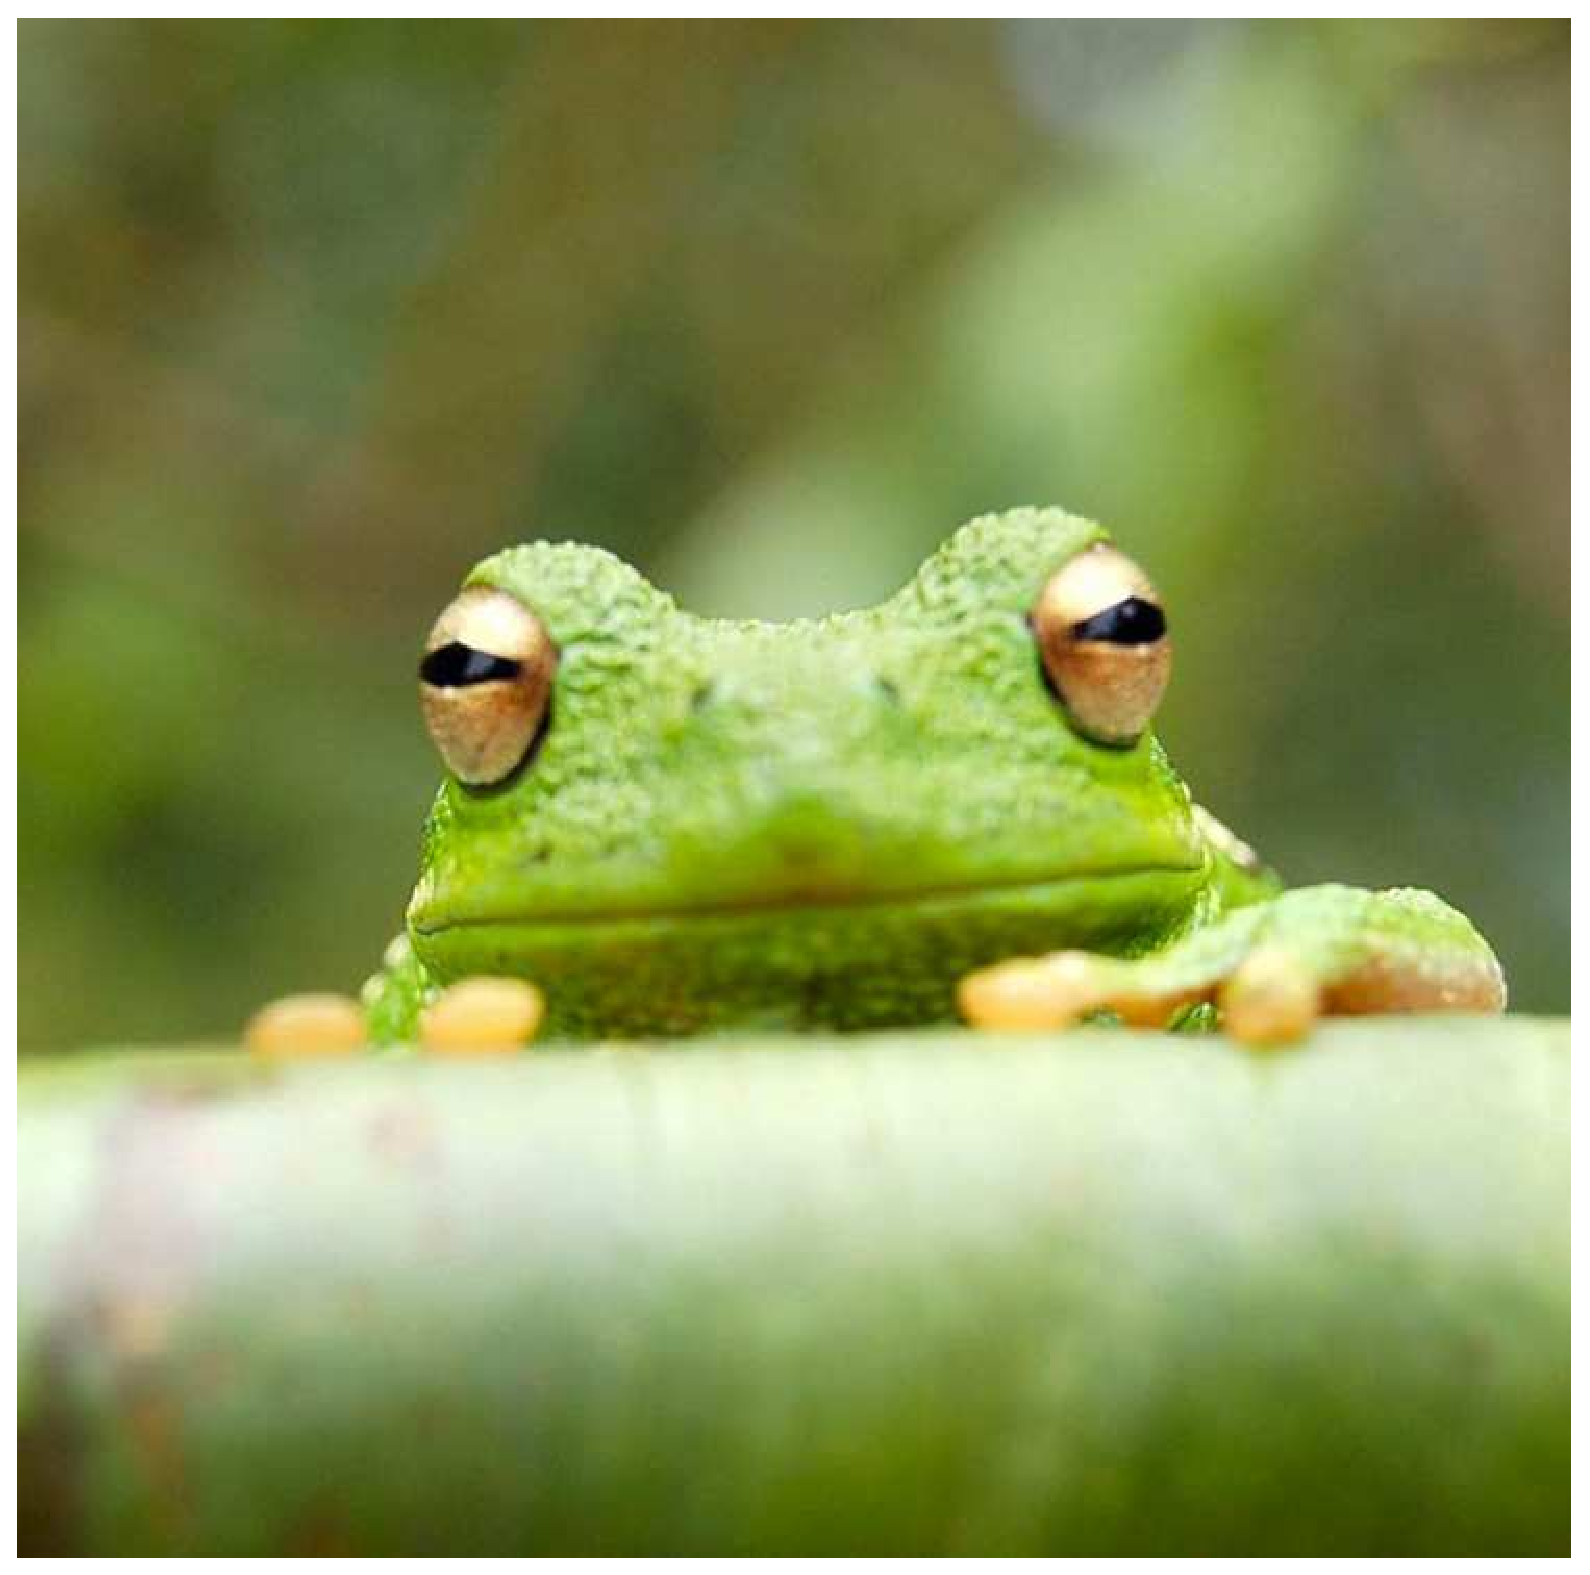
\includegraphics[width=\linewidth,height=7cm]{frog}
% \captionof{figure}{This is a figure in the appendix}
% \end{center}

% \section{Secondly}

% \lipsum[5-8]

% \begin{center}
% 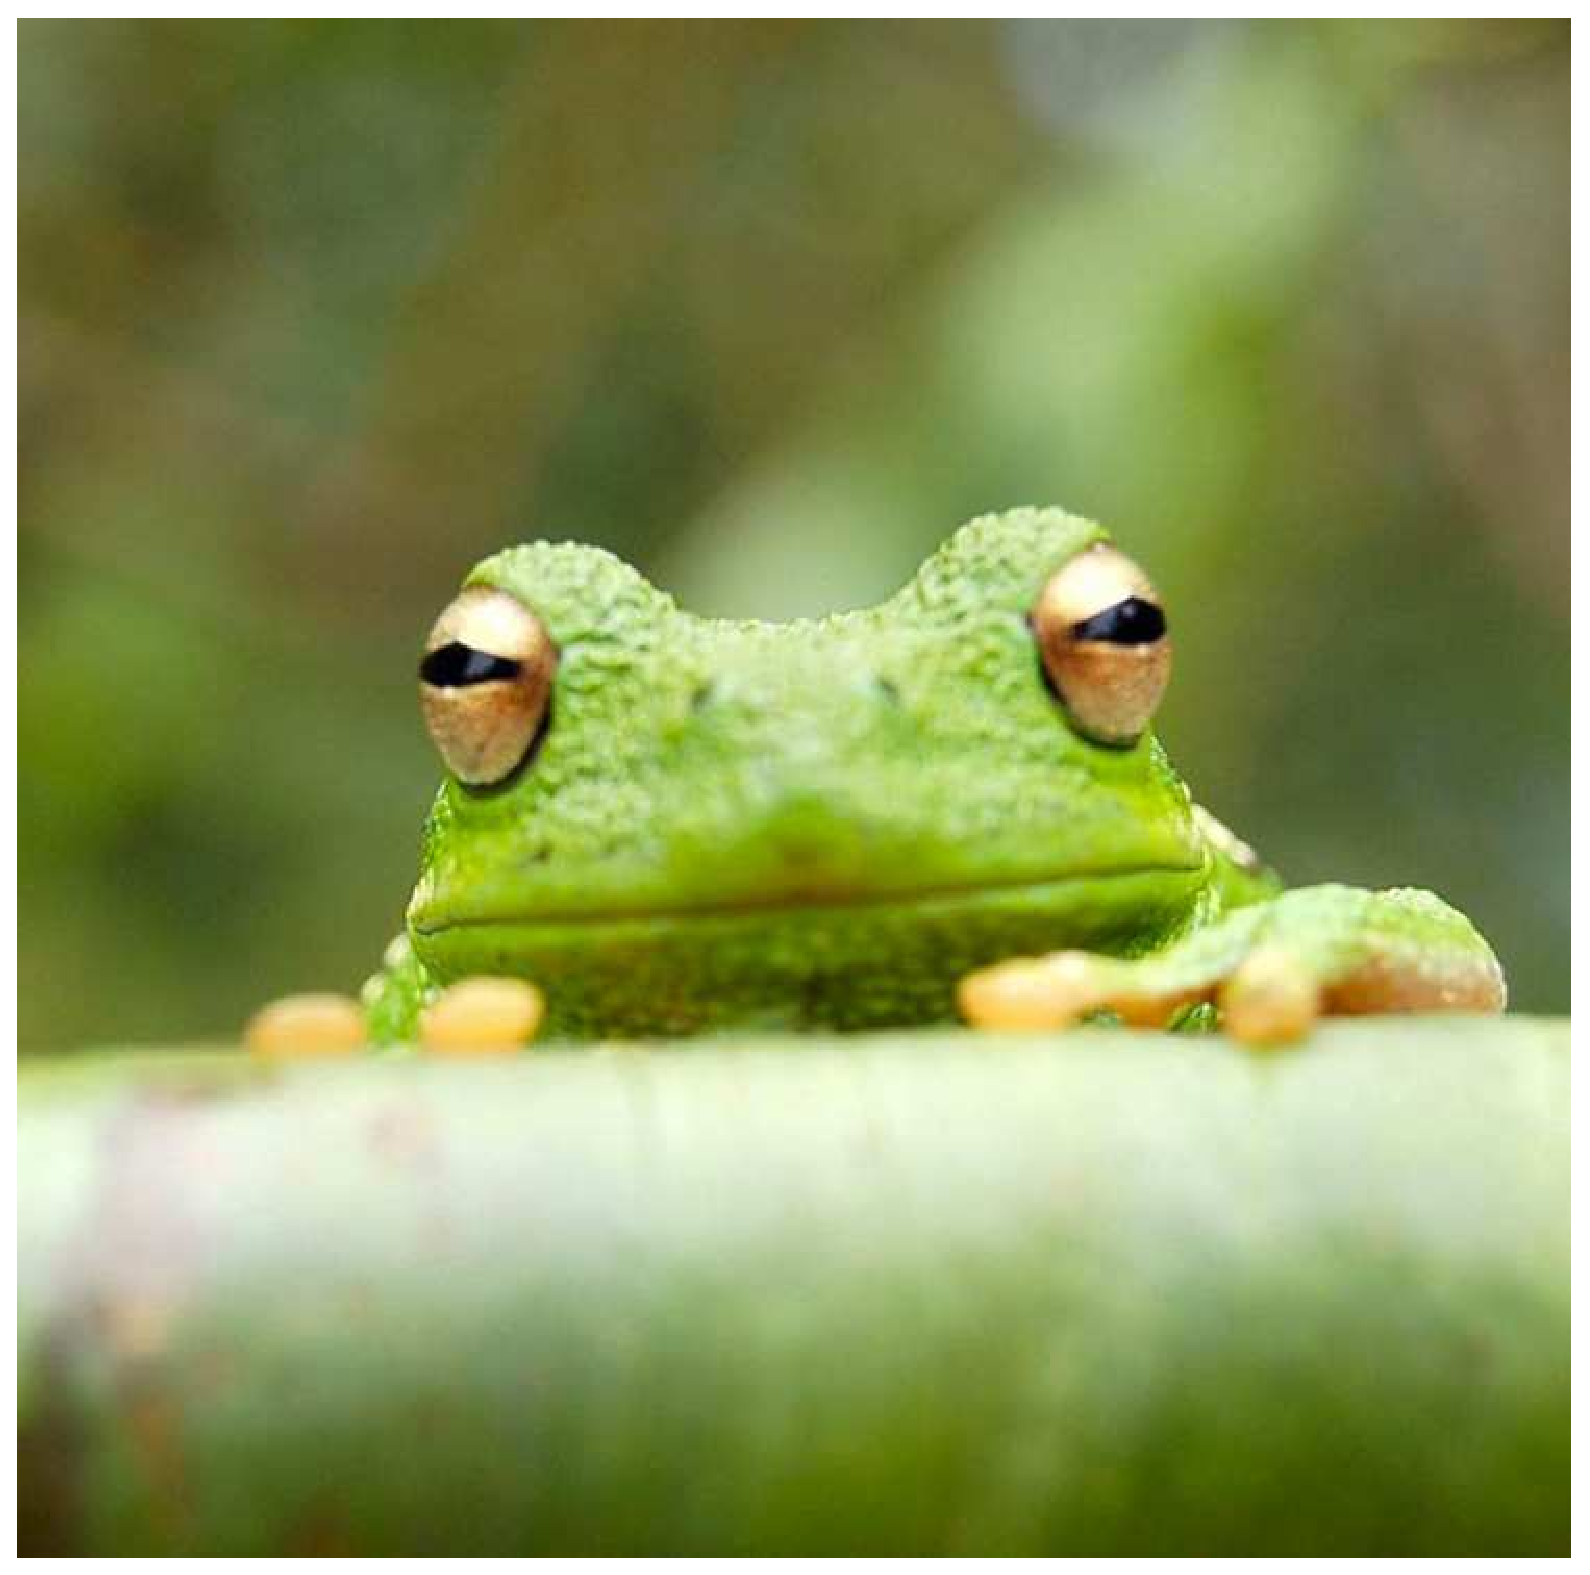
\includegraphics[width=\linewidth,height=7cm]{frog}
% \captionof{figure}{This is a figure in the appendix}
% \end{center}

% \end{appendixbox}

% \begin{appendixbox}
% 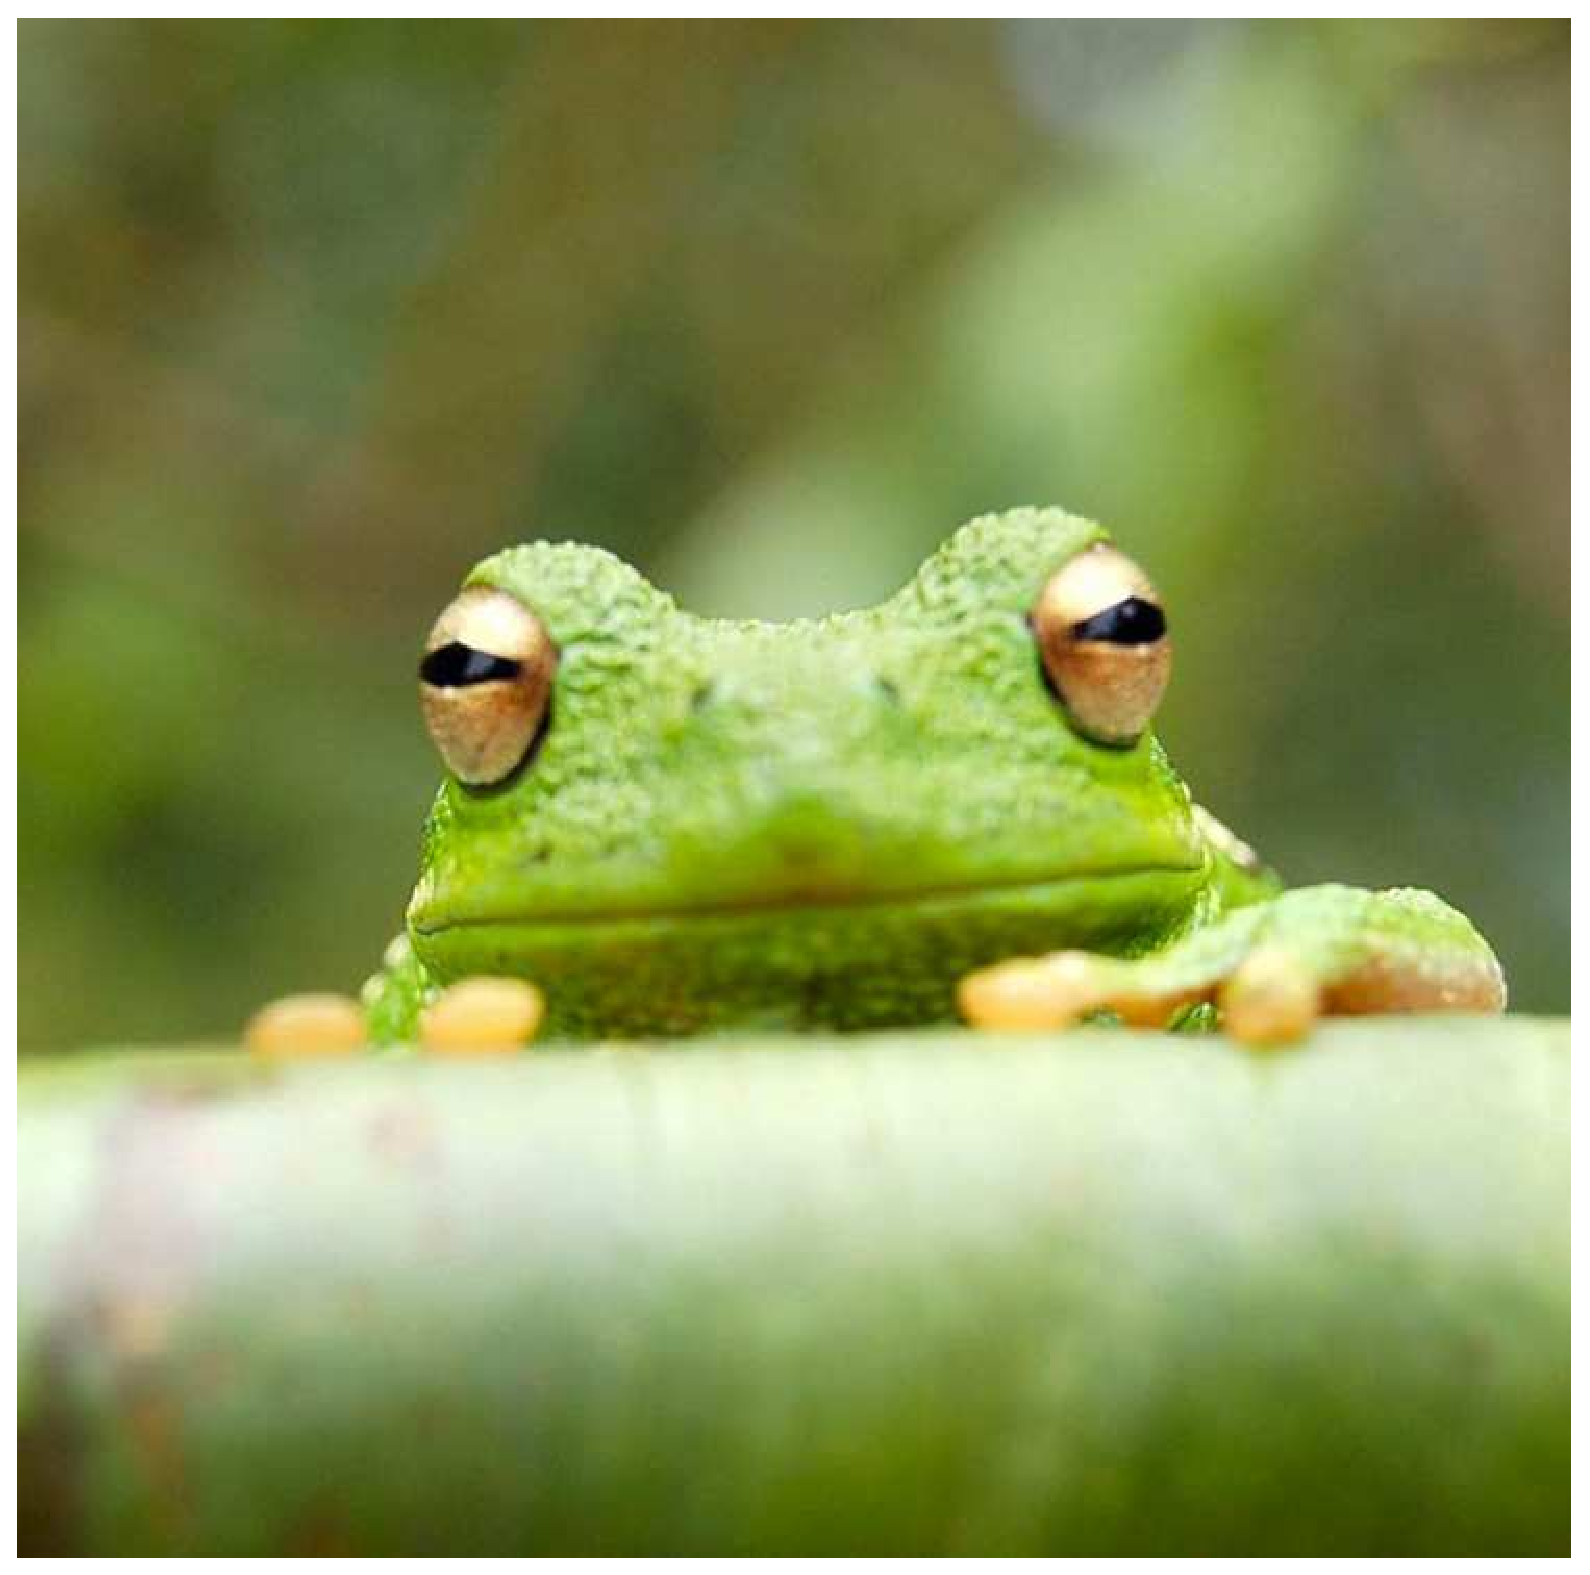
\includegraphics[width=\linewidth,height=7cm]{frog}
% \captionof{figure}{This is a figure in the appendix}
% \end{appendixbox}

\end{document}